% Self-contained Paper C source for the Codex editor and Overleaf.
% Preamble embedded from the shared preamble; no external input or image files required.
% IEEEtran conference class; compiles on Overleaf without modification.
\documentclass[conference]{IEEEtran}
\IEEEoverridecommandlockouts

\usepackage{cite}
\usepackage{amsmath,amssymb,amsfonts}
\usepackage{amsthm}
\usepackage{algorithm}
\usepackage{algorithmic}
\usepackage{graphicx}
\usepackage{textcomp}
\usepackage{xcolor}
\usepackage{booktabs}
\usepackage{url}
\usepackage[hidelinks]{hyperref}
% Lean names carry subscript digits (e.g. frozenGameC₀); the text fonts lack the glyph.
\usepackage{newunicodechar}
\newunicodechar{₀}{\textsubscript{0}}

\def\BibTeX{{\rm B\kern-.05em{\sc i\kern-.025em b}\kern-.08em T\kern-.1667em\lower.7ex\hbox{E}\kern-.125emX}}

\newtheorem{theorem}{Theorem}
\newtheorem{lemma}[theorem]{Lemma}
\newtheorem{proposition}[theorem]{Proposition}
\newtheorem{corollary}[theorem]{Corollary}
\theoremstyle{definition}
\newtheorem{definition}[theorem]{Definition}
\newtheorem{remark}[theorem]{Remark}
\newtheorem{example}[theorem]{Example}

% A machine-checked statement carries its Lean declaration name.
\newcommand{\lean}[1]{\textsf{\footnotesize #1}}
\newcommand{\leanbox}[1]{%
  \par\vspace{2pt}\noindent
  {\raggedright\footnotesize\textsf{Lean: #1}\par}\vspace{2pt}}

% Evidence classes, used consistently and never interchangeably.
\newcommand{\PROVED}{\textsc{proved}}
\newcommand{\CERT}{\textsc{certificate}}
\newcommand{\NUM}{\textsc{numerical}}
% figures resolve both in the repository layout and in a flat Overleaf bundle
\usepackage{pgfplots}
\usepgfplotslibrary{groupplots}
\pgfplotsset{compat=1.17}
\definecolor{cblue}{HTML}{0072B2}
\definecolor{corange}{HTML}{D55E00}
\definecolor{cgreen}{HTML}{009E73}
\definecolor{cpurple}{HTML}{7851A9}
\definecolor{cred}{HTML}{B23A48}
\definecolor{cteal}{HTML}{56B4E9}
\setlength{\emergencystretch}{1em}

% ---------------------------------------------------------------------------
% Draft notes.  Blue is information carried forward for the final write-up;
% red is a decision or a gap that still needs an author.  Both disappear from
% the whole document with one line -- put \shownotesfalse here when the draft
% becomes the submission, and nothing else has to be edited.
% ---------------------------------------------------------------------------
\newif\ifshownotes\shownotestrue
\definecolor{notecol}{RGB}{0,70,190}
\definecolor{todocol}{RGB}{190,20,20}
\newcommand{\NOTE}[1]{\ifshownotes{\color{notecol}\,\textsf{\footnotesize[N: #1]}}\fi}
\newcommand{\TODO}[1]{\ifshownotes{\color{todocol}\,\textsf{\footnotesize[TODO: #1]}}\fi}
% a standalone paragraph-level note, for longer remarks between paragraphs
\newcommand{\NOTEPAR}[1]{\ifshownotes\par\vspace{2pt}\noindent%
  {\color{notecol}\textsf{\footnotesize\textbf{Note.}\;#1}}\par\vspace{2pt}\fi}
\newcommand{\TODOPAR}[1]{\ifshownotes\par\vspace{2pt}\noindent%
  {\color{todocol}\textsf{\footnotesize\textbf{To decide.}\;#1}}\par\vspace{2pt}\fi}


\begin{document}

\title{Exact Marginal--Regret Frontiers\\for Signed-Prefix Compression}

\author{\IEEEauthorblockN{Vu Phan An Nguyen}
\IEEEauthorblockA{\textit{Rider University} \\
Lawrenceville, NJ, USA}}

\maketitle

\begin{abstract}
One random removal order may have to serve every compression budget, while each item must
have nearly uniform probability of removal at every prefix. We determine the price of this
constraint for a signed-weight family, using regret against the best subset at each budget.
For every size $m\ge3$ and every marginal-band width, we obtain the exact minimax expected regret.
With even size $m$, it is
$\max\{2/[(m+4)(m-1)],\,4(1-\eta)/[m(m+4)]\}$.
With odd size it has two affine pieces before reaching the unconstrained value at $\eta=1$.
Exact uniformity costs less than a factor two in even size but a factor proportional to $m$
in odd size. Explicit distributions attain the bounds simultaneously at all budgets; a
composition-flow formulation preserves both the objective and every item marginal.
The timing of the budget changes the answer: choosing it after the order is drawn
multiplies the free value by $m-1$, but the marginal constraint then costs at most $1+1/m$.
On the family and on $(a,-a,b,-b)$, knowing the budget before acting helps only once the band
is loose. On the family it gains
nothing up to the even breakpoint and the odd crossing point; on four items it gains nothing up
to $\eta=1/3$. One exchange after the budget is revealed recovers the whole gain, on four items
and, in even size, on the family at every band.
For arbitrary weight perturbations we prove a Lipschitz bound with recomputed baselines and
normalisation. In odd size, the infimum price ratio over an $\ell_1$ ball of radius
$0<\varepsilon\le1/6$ is $\Theta(\min\{m,1/\varepsilon\})$, with absolute constants.
This is a sharp scale for the erosion of a uniform guarantee, not a claim that every
perturbation destroys the parity effect. The core frontier, attainability, flow and stability
results have Lean~4 proofs, and so does the robust-ball statement.
For every nonzero multiset with $d$ weight types the value equals that of a flow program
on at most $\prod_\tau(n_\tau+1)$ count states. Four two-magnitude count patterns have exact
frontiers at every magnitude ratio and band, with changes in the active certificates. The band is free exactly from an attained threshold
$\eta_{\rm free}$ computed by that program, and the additive price, unlike the ratio, is stable
with no lower bound on the free value.
Stored optimisation certificates and perturbation results provide finite-instance checks.
\end{abstract}

\begin{IEEEkeywords}
ranking under constraints, prefix regret, linear programming duality, formal verification
\end{IEEEkeywords}

\section{Introduction}
\label{sec:intro}

\subsection{The question}

A compressed representation may have to serve a retention budget that is not known in advance. One way to
serve it is as a \emph{removal order}. The system returns an order of the items, and a
consumer who must shed $k$ of them drops the first $k$ and keeps the other $m-k$. Fairness or
exposure requirements then constrain the distribution of the order: each item should be
dropped about equally often at every budget. We ask what that constraint costs when the order
must be good at every budget simultaneously.

Fix $m\ge3$, nonzero weights $g=(g_{1},\dots,g_{m})$ and a normaliser $D>0$. For an order $\pi$ and a budget
$k$, the best achievable loss and the regret are
\begin{equation}
b_{k}(g)=\min_{|S|=k}\Bigl|\sum_{i\in S}g_{i}\Bigr|,\qquad
r_{k}(\pi;g)=\frac{\bigl|\sum_{\ell\le k}g_{\pi_{\ell}}\bigr|-b_{k}(g)}{D}.
\label{eq:regret}
\end{equation}
Here $\{\pi_{1},\dots,\pi_{k}\}$ is the \emph{dropped} set. In the physical model of the
compression, keeping the complement of a set $S$ costs $|\sum_{i\in S}g_{i}|/2$. So with
$D=\|g\|_{1}$, the regret~\eqref{eq:regret} is the loss of the compression that keeps the
last $m-k$ items, above the best compression of that size, normalised by $\|g\|_{1}/2$.

\leanbox{\lean{physical\_radius}, \lean{physical\_minimum}, \lean{physical\_normalized\_regret}
in \lean{LeanPaperCStabilityEndgameV1}}

For a distribution $P$ over orders, the constrained optimum is
\begin{equation}
V_{g}(\eta)=\inf_{P}\ \max_{0<k<m}\ \mathbb{E}_{\pi\sim P}\,r_{k}(\pi;g)
\label{eq:value}
\end{equation}
subject to the marginal band
\begin{equation}
\Bigl|\Pr\nolimits_{P}\bigl(i\in\{\pi_{1},\dots,\pi_{k}\}\bigr)-\frac{k}{m}\Bigr|\le\frac{\eta}{m}
\quad(\text{all }i,\ k\le m).
\label{eq:band}
\end{equation}
The band reads the same whether it is stated for dropping or for keeping. An item is kept at
size $m-k$ with probability within $\eta/m$ of $\frac{m-k}{m}$ exactly
when~\eqref{eq:band} holds. The budget in~\eqref{eq:value} is fixed before the draw, so the
objective is $\max_{k}\mathbb{E}\,r_{k}$. Section~\ref{sec:expost} treats the objective
$\mathbb{E}\max_{k}r_{k}$, where the budget is chosen after the draw. The two objectives are
never interchanged.

\subsection{Contributions at a glance}

We work on the family $g_{m}$ of~\eqref{eq:family} below. We write
$V_{m}(\eta)=V_{g_{m}}(\eta)$ and $V^{\mathrm{free}}_{m}=\frac{2}{(m+4)(m-1)}$. The latter is
the unconstrained optimum, because the band is vacuous for $\eta\ge m$.

\begin{enumerate}
\item[1)] \textbf{The whole frontier} (Theorems~\ref{thm:zero}, \ref{thm:even},
\ref{thm:odd}). $V_{m}(\eta)$ in closed form for every $m\ge3$ and every $\eta\ge0$. At
$\eta=0$ the price $V_{m}(0)/V^{\mathrm{free}}_{m}$ is $\frac{2(m-1)}{m}<2$ in even size and
$\frac{(m+3)(m-1)}{2m}$ in odd size. The premium over one vanishes exactly at $\eta_{*}=\frac{m-2}{2(m-1)}$
(even) and at $\eta_{*}=1$ (odd).
\item[2)] \textbf{A polynomial-size program with the same value} (Theorem~\ref{thm:flow}).
\item[3)] \textbf{Robustness, and where it ends} (Theorems~\ref{thm:robust},
\ref{thm:collapse}, Corollary~\ref{cor:robustball}). A Lipschitz envelope for arbitrary
weights, and a two-sided law for the smallest price ratio in an $\ell_1$ ball:
$\Theta(\min\{m-1,1/\varepsilon\})$ for $0<\varepsilon\le1/6$.
Radius $1/m$ marks when a linear-in-$m$ price ceases to be guaranteed uniformly;
some much larger perturbations preserve it exactly.
\item[4)] \textbf{Any number of types} (Theorems~\ref{thm:typedflow}, \ref{thm:freeband},
\ref{thm:twomag}, \ref{thm:twomag2211}, \ref{thm:twomagprice}, \ref{thm:twomag1122},
\ref{thm:twomag2222}, Proposition~\ref{prop:gap}). For every multiset with $d$ weight types the flow program has the
same value over at most $\prod_\tau(n_\tau+1)$ count states. The band is free exactly from a threshold
$\eta_{\rm free}$, which is attained and read off that program. The additive price
$V_g(\eta)-V^{\rm free}_g$ is $6/\nu$-Lipschitz in $\ell_1$ on multisets with $\|g\|_1\ge\nu>0$, with
no lower bound on the free value.
On $(a,-a,b,-b)$ and on counts $(2,2,1,1)$ the normalised frontier $V_g/V_g^{\rm free}$ is the same at
every ratio. On counts $(1,1,2,2)$ and $(2,2,2,2)$ the whole frontier is exact, its free threshold moves with
$a/b$, and the price is not monotone in $a/b$.
\item[5)] \textbf{Timing} (Proposition~\ref{prop:expost}, Theorem~\ref{thm:expostband}).
Choosing the budget after the draw multiplies the free value by $m-1$. Under the band the
ex-post value is known exactly, and there the band costs at most a factor $1+\frac1m$.
\item[6)] \textbf{Knowing the budget, and one exchange} (Proposition~\ref{prop:sandwich},
Theorems~\ref{thm:zerovalue}, \ref{thm:awareexact}, \ref{thm:fourrecourse}). A policy that learns
the budget first is never worse, and $\lfloor m/2\rfloor$ exchanges after the reveal reach it. On
$g_m$ its value is exact at every band: it gains nothing up to the even breakpoint and the odd
crossing point, and it gains past them; in even size one exchange recovers the whole gain at
every band. On $(a,-a,b,-b)$ it gains nothing up to $\eta=\frac13$, and one exchange recovers the
whole gain.
\end{enumerate}

\subsection{Prior work, and what does not follow from it}

Randomised rankings with constrained position or exposure marginals are a studied object.
Singh and Joachims~\cite{singh2018} introduce exposure constraints and optimise a linear
utility over the Birkhoff polytope. Celis, Straszak and Vishnoi~\cite{celis2018} bound group
representation in every prefix. Singh, Kempe and Joachims~\cite{singh2021} constrain, for every
item and every $k$, the probability that the item is ranked in the top $k$, and contrast ex-ante
and ex-post guarantees, as Freeman, Shah and Vaish~\cite{freeman2020} do in allocation. We
take that framing as given. We do not claim the flow technique either: reducing a permutation
polytope to a compositions DAG is standard~\cite{schrijver2003}. One ordering that serves every
budget is the object of incremental maximization, with competitive ratios for monotone
objectives~\cite{disser2023,bienkowski2026}. Storandt and Funke~\cite{storandt2019} explicitly
study regret-minimizing permutations, minimizing accumulated average regret over prefixes;
their Theorem~16 gives a greedy approximation for accumulated happiness. Prefix-constrained
ranking also includes closest-ranking problems under flag matroid constraints~\cite{ando2026}.
Signed-prefix control has precedents in discrepancy and the Steinitz rearrangement problem;
prefix discrepancy chooses signs for a given vector sequence~\cite{bansal2021}, whereas here
the signed weights are fixed and the order law is chosen. Choosing dependence under fixed
marginals to control sums over unknown subsets is studied through joint mixes~\cite{koike2022}.
Discrete mixability also optimizes column permutations and uses maximum flow for restricted
integer matrices~\cite{bellini2016}.

What is new is the law that the reduction lets us prove, for an objective these works do not
treat. The signed-prefix regret is an absolute sum net of the per-budget optimum, taken at
every budget. It is not linear in the order, and the parity of $k$ enters through $b_{k}$. It
depends on the joint law of each prefix, not only on the position marginals. With weights
$(+1,+1,-1,-1)$ on items $1,2,3,4$, the four cyclic shifts of the order $(1,3,2,4)$, with signs
$(+,-,+,-)$, and the four cyclic shifts of $(1,2,3,4)$, with signs $(+,+,-,-)$, each put every item
at every position with probability $\frac14$. Their expected $|\text{prefix}_{2}|$ are $0$ and
$1$. So the marginal rank matrix, which suffices for a linear utility, does not
suffice here. Against incremental maximization, the values here are exact minimax values under
marginal bands with signed cancellation and a per-budget optimum, not competitive ratios. The
cited joint-mix results do not yield these frontiers: their robust subset-sum formulation
optimizes over couplings with prescribed marginals, with exact quadratic-cost results under
symmetric subset uncertainty~\cite{koike2022}. Our feasible laws instead preserve the full
multiset in each realization, enforce nested prefixes and item bands, and use absolute-sum
regret relative to a different optimum at each budget. This is a distinction between the
specified problems, not a claim that permutation constructions are absent from mixability.

Limited revision after uncertainty is revealed is also established machinery. Recoverable
selection permits exchanges after costs are revealed~\cite{chassein2017}; recoverable
optimization with commitment instead preserves surviving elements after deletions~\cite{hommelsheim2026}.
Online discrepancy studies repeated sign changes under arrivals and deletions~\cite{gupta2022}.
Here weights are known, the revealed quantity is the budget, and the initial law must serve
all budgets with both initial and final item bands. Our recourse contribution is the exact
onset of the commitment gap and its complete recovery by one exchange on the stated families,
not the two-stage recovery framework itself.

\begin{table}[h]
\caption{Closest research threads and the specific quantitative results compared here.}
\label{tab:prior}
\centering
\footnotesize
\begin{tabular}{@{}p{0.30\columnwidth}p{0.62\columnwidth}@{}}
\toprule
Nearest source & Specific result compared here \\
\midrule
Exposure-constrained rankings~\cite{singh2018} & The exact signed-prefix frontier at every
size and band, with a $\Theta(m)$ parity split (Thms.~\ref{thm:zero}--\ref{thm:odd}) \\
Prefix-fair ranking~\cite{celis2018} & The exact breakpoints and the crossing point
$\eta_{t}$ of the odd frontier (Thm.~\ref{thm:odd}) \\
Ex-ante vs.\ ex-post~\cite{singh2021,freeman2020} & The exact banded ex-post value, and the
fact that the band and timing prices do not multiply (Thm.~\ref{thm:expostband}) \\
Flow reductions~\cite{schrijver2003} & Value equality with every per-item band carried
through relabelling, for every typed multiset over $\prod_\tau(n_\tau+1)$ states, and the free
threshold read off it (Thms.~\ref{thm:flow}, \ref{thm:typedflow}, \ref{thm:freeband}) \\
Prefix regret~\cite{storandt2019,disser2023,bienkowski2026} & Exact values, not ratios, under
marginal bands and signed cancellation (Thms.~\ref{thm:zero}--\ref{thm:odd}) \\
Joint mixes~\cite{koike2022,bellini2016} & The prefix-nested, permutation-restricted frontiers
(Thms.~\ref{thm:zero}--\ref{thm:odd}) \\
Recoverable selection~\cite{chassein2017,hommelsheim2026} & The exact value of knowing the budget, and of one exchange after it
is revealed (four items; $g_m$ in even size), under marginal bands (Thms.~\ref{thm:zerovalue},
\ref{thm:awareexact}, \ref{thm:fourrecourse}) \\
\bottomrule
\end{tabular}
\end{table}

\subsection{Evidence and formal scope}

Three evidence classes appear, and they are never interchanged.
\begin{itemize}
\item \PROVED: a theorem stated at the paper's objects and checked in
Lean~4~\cite{demoura2021} against Mathlib~\cite{mathlib2020}.
\item \CERT: an exact rational certificate verified by a script.
\item \NUM: a floating-point solve or search.
\end{itemize}
Each formal theorem carries a line naming its Lean declaration. The robust-ball corollary
is proved in this text and checked as \lean{robust\_ball}. The proof architecture and supporting
declarations are in the supplement. Audited modules use no \texttt{sorry} or
\texttt{native\_decide}, and their axioms lie within \{\texttt{propext},
\texttt{Classical.choice}, \texttt{Quot.sound}\}. A compiled theorem certifies its statement
under its hypotheses. Every hypothesis of a headline is either a model assumption displayed
in it or discharged.

\section{Setting}
\label{sec:setting}

\paragraph{Compression model and scope}
The signed-prefix objective has an exact compression interpretation on a shared binary
support. Let $Q_i(z)=g_i z$ for $z\in\{0,1\}$ and $F_g(z)=\sum_iQ_i(z)$.
If $S$ is removed, the retained representation is $\sum_{i\notin S}Q_i(z)$ plus a constant
chosen to minimise worst-case error. Thus
\begin{equation}
\begin{aligned}
L_g(S)&=\inf_{c\in\mathbb R}\max_{z\in\{0,1\}}
\left|z\sum_{i\in S}g_i-c\right|\\
&=\frac12\left|\sum_{i\in S}g_i\right|.
\end{aligned}
\label{eq:physicalmodel}
\end{equation}
Subtracting the best loss among $k$-sets and dividing by $\|g\|_1/2$ gives
\eqref{eq:regret}. All normalised statements assume $\|g\|_1>0$.
The shared support permits signed cancellation; this interpretation does not assert the
same loss for arbitrary independent inputs or arbitrary learned compression models.
The mathematical ranking problem is defined directly by~\eqref{eq:regret}--\eqref{eq:band}.
Throughout, $\eta\ge0$ and budgets are $0\le k\le m$, with the objective on $0<k<m$.

\paragraph{The parity family}
The family studied throughout is
\begin{equation}
g_{m}=\bigl(-3,\underbrace{-1,\dots,-1}_{p},\underbrace{1,\dots,1}_{q},3\bigr),
\qquad D=m+4,
\label{eq:family}
\end{equation}
with $p=\lceil\frac{m-2}{2}\rceil$ and $q=\lfloor\frac{m-2}{2}\rfloor$. The total is $0$ for
even $m$ and $-1$ for odd $m$, and $\|g_{m}\|_{1}=m+4=D$. Every weight is an odd integer, so
a sum of $k$ weights has the parity of $k$ and has absolute value at least $k\bmod2$. For
$g_{m}$ the per-budget optimum is exactly that,
\begin{equation}
b_{k}(g_{m})=k\bmod 2\qquad(0<k<m),
\label{eq:baseline}
\end{equation}
attained by an explicit subset at each budget. So on $g_{m}$ the physical regret, with the
baseline computed from its definition, is the normalised parity excess.

\leanbox{\lean{familyBaselineIdentification\_holds} in \lean{LeanPaperCBaselineAttainV1};
\lean{trueValue\_family} in \lean{LeanPaperCStabilityFamilyV1}}

The parity split lives on this structure. There are two heavy items of weight $\pm3$, and
light items of weight $\pm1$ whose counts differ by one in odd size. A $+3$ step between two
budgets of zero excess is impossible, because a zero-excess prefix sum has absolute value at
most $1$. That observation drives every odd lower bound below.

\section{Methodology: exact reduction and matching certificates}
\label{sec:flow}

Our method has two stages. First, we replace a distribution over permutations by a flow
without changing any feasible budget vector. Second, we bound its minimax objective from
below by certificates and attain each bound with an explicit law. Numerical solves help
locate candidate regimes; the exact identities below are established by those two sides.

\subsection{From item marginals to a flow}

The direct formulation has $m!$ order variables. After symmetrisation, a prefix is characterised,
both for the objective and for the band, by its composition
$v=(n_{-3},n_{-1},n_{+1},n_{+3})\le(1,p,q,1)$. There are $4(p+1)(q+1)=O(m^{2})$ of them. Let
$\mathcal{F}_{m}(\eta)$ be the unit flows on the layered DAG of compositions whose edges add
one item, with the band imposed on the class occupancies.

\begin{theorem}[Flow equivalence]
\label{thm:flow}
Fix $m\ge3$, $\eta\ge0$, and a functional $\Phi$ of the budget vector $(\mathbb{E}r_{k})_{k}$. The
infimum of $\Phi$ over band-feasible laws on all $m!$ orders of $g_{m}$ equals its infimum
over $\mathcal{F}_{m}(\eta)$. In particular $V_{m}(\eta)$ is the value of the flow program,
and Theorems~\ref{thm:even} and~\ref{thm:odd} hold for it.
\end{theorem}

\leanbox{\lean{actual\_banded\_infima} in \lean{LeanPaperCFlowBandJoinV1};
\lean{odd\_frontier} in \lean{LeanPaperCOddFrontierV1}; \lean{support\_box} in
\lean{LeanPaperCFreeBandV1}; \lean{value\_eq\_flow}, \lean{even\_frontier\_flow}, \lean{odd\_breakpoint\_flow} in
\lean{LeanPaperCFlowObjectiveV1}}

Three maps make it exact.
\begin{itemize}
\item A law induces the occupancy of each composition. Conservation is the consistency of the
marginals of one joint law.
\item Averaging over relabellings inside a weight class keeps every $r_{k}$. It replaces each
item's marginal by its class average.
\item A unit flow carries a Markov law on whole trajectories. A trajectory of positive mass is
a sequence of one-item steps, hence the layer map of an actual order. Relabelling within
classes then recovers the per-item band.
\end{itemize}
The two programs reach exactly the same set of budget vectors, and that set is non-empty for
every $\eta\ge0$. The statement concerns the value of the four-type program on $g_{m}$. It
gives no algorithm for perturbed weights.

\begin{table}[t]
\caption{Flow-program sizes against the order formulation. \NUM{}}
\label{tab:agree}
\centering
\footnotesize
\begin{tabular}{@{}rrrl@{}}
\toprule
$m$ & flow states & flow edges & orders \\
\midrule
$11$ & $120$ & $316$ & $13{,}860$ type sequences \\
$15$ & $224$ & $612$ & intractable \\
$21$ & $440$ & $1236$ & intractable \\
$31$ & $960$ & $2756$ & intractable \\
\bottomrule
\end{tabular}
\end{table}


\subsection{The optimisation and its certificates}
For type counts $n_\tau$, write
$\mathcal C_k=\{v:0\le v_\tau\le n_\tau,\ \sum_\tau v_\tau=k\}$.
Let $x_k(v)$ be the probability of count state $v$ and $f_k(v,v+e_\tau)$ its outgoing
flow. The program minimises an epigraph variable $t$, subject to nonnegative flows,
$x_0(0)=1$, flow conservation, and
\begin{align}
\left|\sum_{v\in\mathcal C_k}\frac{v_\tau}{n_\tau}x_k(v)-\frac{k}{m}\right|
&\le\frac{\eta}{m},\qquad n_\tau>0,\label{eq:flowband}\\
\sum_{v\in\mathcal C_k}x_k(v)
\frac{|\sum_\tau\mathrm{wt}_\tau v_\tau|-b_k(g)}{D}
&\le t,\qquad 0<k<m.\label{eq:flowobjective}
\end{align}
The first constraint is exactly the per-item band after uniform relabelling within types.
The second keeps a separate expected loss for every budget: taking the maximum is achieved
by $t$, rather than by replacing the objective with an average.

A lower certificate combines nonnegative budget weights, marginal-band inequalities and
potentials on count states. Its edge inequalities telescope along every path and therefore
bound every feasible law. For the upper side, a finite mixture of type sequences is checked
for its mass, every marginal band, and every budget cost. Uniform relabelling lifts that
mixture to actual item permutations. Equality of the lower certificate and upper value proves
optimality over all orders, rather than only over the displayed construction.
\leanbox{\lean{potential\_bound}, \lean{band\_sum}, \lean{cert\_lower} in
\lean{LeanPaperCFlowCertV1}; the item-level lift is Theorem~\ref{thm:flow}.}

\subsection{How a whole frontier is obtained}
For fixed weights, each certificate gives an affine lower bound in $\eta$; the free value is
another lower bound. If two laws meet the active bound at $\eta_0$ and $\eta_1$, their mixture
with weight $(\eta-\eta_0)/(\eta_1-\eta_0)$ is feasible at every intermediate band and has
budget costs interpolating between the endpoints. This proves the segment without fitting
an LP grid. When the weights vary, baseline changes and competing certificates divide the
magnitude ratio into regions. We prove coverage of the regions and check the shared
endpoints, including coincident kinks.
\leanbox{\lean{up\_seg}, \lean{regions\_cover} in \lean{LeanPaperCTwoMag1122FrontierV1};
\lean{up\_seg8}, \lean{regions8\_cover} in \lean{LeanPaperCTwoMag2222FrontierV1}.}

The following sections use this method to answer three distinct questions: the price of a
universal order, its sensitivity to the weights, and the effect of revealing the budget
before or after that order is drawn. Their quantifiers are kept separate.

\section{Main results: the parity frontier}
\label{sec:frontier}

\begin{theorem}[Zero band]
\label{thm:zero}
For every even $m\ge4$ and every odd $m\ge3$,
\[
V_{m}(0)=
\begin{cases}
\dfrac{4}{m(m+4)}, & m\text{ even},\\[8pt]
\dfrac{m+3}{m(m+4)}, & m\text{ odd},
\end{cases}
\]
attained by an explicit law on all $m!$ orders of $g_{m}$. Hence
$V_{m}(0)/V^{\mathrm{free}}_{m}$ is $\frac{2(m-1)}{m}$ for even $m$ and
$\frac{(m+3)(m-1)}{2m}$ for odd $m$.
\end{theorem}

\leanbox{\lean{even\_value\_zero}, \lean{odd\_value\_zero}, \lean{odd\_uniform\_price\_ratio}
in \lean{LeanPaperCEndgameV1}; \lean{even\_allPerm\_witness} in \lean{LeanPaperCEvenWitnessJoinV1};
\lean{odd\_allPerm\_witness} in \lean{LeanPaperCOddWitnessJoinV1}}

\begin{theorem}[The even frontier]
\label{thm:even}
For every even $m\ge4$ and every $\eta\ge0$,
\[
V_{m}(\eta)=\max\Bigl\{\frac{2}{(m+4)(m-1)},\ \frac{4(1-\eta)}{m(m+4)}\Bigr\},
\]
so the marginal constraint becomes free exactly at $\eta_{*}=\frac{m-2}{2(m-1)}$.
\end{theorem}

\leanbox{\lean{even\_frontier\_all} in \lean{LeanPaperCEndpointLawV1}}

\begin{theorem}[The odd frontier]
\label{thm:odd}
For every odd $m\ge3$ and every $\eta\ge0$,
\begin{multline*}
V_{m}(\eta)=\max\Bigl\{\frac{m+3-(m+1)\eta}{m(m+4)},\\
\frac{2}{(m+4)(m-1)}+\frac{(1-\eta)_{+}}{m(m+4)}\Bigr\}.
\end{multline*}
The two lines cross at $\eta_{t}=1-\frac{2}{m(m-1)}$, where
$V_{m}(\eta_{t})=\frac{2(m^{2}+1)}{m^{2}(m-1)(m+4)}$. In particular
$V_{m}(\eta)=V^{\mathrm{free}}_{m}$ exactly when $\eta\ge1$, and for any fixed $\eta<1$ the
odd price is $\Omega(m)$.
\end{theorem}

\leanbox{\lean{odd\_frontier}, \lean{odd\_kink\_value} in \lean{LeanPaperCOddFrontierV1};
\lean{odd\_breakpoint} in \lean{LeanPaperCEndpointLawV1}}

\emph{Why the frontier has this shape.} Every lower side comes from one budget or from an
average of budgets. Every upper side is one explicit law.

\emph{Zero band.} For even $m$ the weights sum to zero, so the prefix of length $m-1$ is minus
the last item. Then $r_{1}+r_{m-1}$ equals $\frac{2}{D}$ times the number of heavy items at
the two ends, and each end is heavy with probability $\frac{2}{m}$. For odd $m$ the prefix
of length $m-1$ is $-1$ minus the last item, and $m-1$ is even, so an item of weight $w$ in
last position costs $\frac{|1+w|}{D}$. Averaging over uniform last positions gives
$\frac{m+3}{mD}$. The upper laws are the following, each relabelled uniformly within weight
classes. For even $m$, the insertion mixture with one flat order. For odd $m$, the uniform
law on the cyclic shifts of $(+3,-3,-1,+1,\dots,-1)$.

\emph{The first odd line.} Only budget $m-1$ is used. By the band at $k=m-1$, the
last-position law satisfies $|\pi_{i}-\frac1m|\le\frac{\eta}{m}$. Hence for any centre $a$,
$\sum_{i}\pi_{i}c_{i}\ge\frac1m\sum_{i}c_{i}-\frac{\eta}{m}\sum_{i}|c_{i}-a|$. With
$c_{i}=|1+g_{i}|$ and $a=2$ the two sums are $m+3$ and $m+1$.

\emph{The second odd line.} Every order pays total excess at least $2+2[\pi_{m}>0]$. The
$+3$ step forces excess $2$ on the two budgets around it, and a positive last item forces two
more at budget $m-1$. The band puts each of the $\frac{m-1}{2}$ positive items last with
probability at least $\frac{1-\eta}{m}$. So the average over budgets, and hence the maximum,
is at least $V^{\mathrm{free}}_{m}+\frac{1-\eta}{mD}$.

\emph{The upper side.} $V_{m}$ is convex in $\eta$, so three laws suffice:
\begin{itemize}
\item the zero-band law at $\eta=0$;
\item the insertion mixture at $\eta=1$, whose value is $V^{\mathrm{free}}_{m}$;
\item a law at the crossing point $\eta_{t}$, with value exactly
$\frac{2(m^{2}+1)}{m^{2}(m-1)D}$.
\end{itemize}
The last law is new. For $m\ge7$ it is a mixture of explicit orders, with masses in units of
$\frac{1}{m^{2}(m-1)}$:
\begin{itemize}
\item mass $m^{2}+1$ on each insertion slot $0,\dots,m-3$ ($m^{2}-m+4$ at slot $0$), split
equally between two versions. Version~A is the insertion order. Version~B is its negation
with the last item set to $-1$;
\item $m(m-1)$ on version~A at slot $m-2$;
\item $2$ on the order that puts the light items of slot $m-2$ first and ends with
$(-3,+3)$;
\item $m-3$ on version~A at slot $0$ with its last two light items swapped, which ends with
$(-1,+1)$.
\end{itemize}
Every budget then carries expected excess exactly $\frac{2(m^{2}+1)}{m^{2}(m-1)}$, and the
class counts of every prefix satisfy the band at $\eta_{t}$. At $m=3$ and $m=5$ an explicit
finite law takes its place.

\section{Any number of weight types}
\label{sec:typed}

Theorem~\ref{thm:flow} uses only one fact about $g_m$: its items fall into weight classes. Let
$g=\mathrm{wt}\circ\mathrm{ty}$ for a type map $\mathrm{ty}:[m]\to[d]$ and type weights
$\mathrm{wt}\in\mathbb R^d$, and let $n_\tau$ be the multiplicity of type $\tau$. A count state
$v\in\prod_\tau[0,n_\tau]$ records how many items of each type the prefix has dropped. Its cost
at budget $k$ is $(|\sum_\tau\mathrm{wt}_\tau v_\tau|-b_k(g))/\|g\|_1$.

\begin{theorem}[The flow program for every typed multiset]
\label{thm:typedflow}
For every type map and weights with $\|g\|_1>0$, and every $\eta\ge0$:
\begin{itemize}
\item on a ranking, the count cost of its prefix composition is its normalised regret;
\item the budget vectors of band-feasible laws over all $m!$ rankings are exactly those of the
count-feasible banded flows, so every functional of the budget vector has the same infimum;
\item a count-feasible flow lives on the box $\prod_\tau[0,n_\tau]$, which has
$\prod_\tau(n_\tau+1)\le(m+1)^d$ states.
\end{itemize}
The reachable states across all layers belong to this box. For a fixed number of types
the program therefore has $O(m^d)$ count states. This is a
polynomial model for each fixed $d$, not a polynomial algorithm for arbitrary weights.
\end{theorem}
\leanbox{\lean{typedCost\_eq}, \lean{typed\_flow\_equivalence}, \lean{typed\_banded\_infima},
\lean{card\_state}, \lean{family\_is\_typed} in \lean{LeanPaperCTypedFlowV1};
\lean{support\_box}, \lean{card\_box} in \lean{LeanPaperCFreeBandV1}}

Flow reductions of permutation problems are not new~\cite{schrijver2003}. The content here is
that a nonlinear prefix objective and every per-item band survive the reduction together.

In this section and in Section~\ref{sec:aware} the normaliser is $D=\|g\|_1$.

\paragraph{When the band is free} The deviation of a law is
$\mathrm{dev}(P)=m\max_{k\le m,\,i}|P(i\text{ in the first }k)-k/m|$, so a law is band-feasible
at $\eta$ exactly when $\mathrm{dev}(P)\le\eta$. The band is vacuous at $\eta=m$, so
$V^{\rm free}_g=V_g(m)$. Let
\[
\eta_{\rm free}(g)=\min\{\mathrm{dev}(P):P\ \text{attains}\ V^{\rm free}_g\}.
\]

\begin{theorem}[The free threshold]
\label{thm:freeband}
Let $\|g\|_1>0$. The value and the threshold are attained. For every $\eta\ge0$,
$V_g(\eta)=V^{\rm free}_g$ if and only if $\eta\ge\eta_{\rm free}(g)$. For a typed multiset
the same holds with $V_g$ replaced by the value of the flow program of
Theorem~\ref{thm:typedflow}. So $\eta_{\rm free}$ is the least $\eta$ at which that program
reaches its value at $\eta=m$.
\end{theorem}
\leanbox{\lean{feasible\_iff\_dev}, \lean{feasible\_m\_eq}, \lean{attain\_value},
\lean{attain\_eta}, \lean{free\_threshold}, \lean{trueValue\_eq\_flow}, \lean{free\_threshold\_flow}
in \lean{LeanPaperCFreeBandV1}}

Stated for laws alone, the threshold is close to a definition. The flow form is what makes it a
computation: one parametric program over at most $\prod_\tau(n_\tau+1)$ count states. On
$g_m$ Theorems~\ref{thm:even} and~\ref{thm:odd} give it in closed form:
$\eta_{\rm free}=\frac{m-2}{2(m-1)}$ in even size and $1$ in odd size.

\paragraph{The additive price} Let $\Delta_g(\eta)=V_g(\eta)-V^{\rm free}_g$.

\begin{proposition}[The additive price is stable]
\label{prop:gap}
Let $\|g\|_1>0$ and $\eta\ge0$. Then $\Delta_g(\eta)\ge0$, $\Delta_g$ is nonincreasing, and
$\Delta_g(\eta)=0$ exactly when $\eta\ge\eta_{\rm free}(g)$. For all $g,g'$ with
$\|g\|_1,\|g'\|_1\ge\nu>0$,
\[
|\Delta_g(\eta)-\Delta_{g'}(\eta)|\le6\|g-g'\|_1/\nu.
\]
\end{proposition}
\leanbox{\lean{gap\_nonneg}, \lean{gap\_antitone}, \lean{gap\_zero\_iff}, \lean{gap\_stable} in
\lean{LeanPaperCFreeBandV1}}

The ratio $V_g(0)/V^{\rm free}_g$ needs $V^{\rm free}_g>0$, and it can blow up when the free
value is small. The additive price needs no such condition. In the exploration below, $96$ of the
$240$ (count vector, ratio) instances have $V^{\rm free}_g=0$ to solver precision \NUM. There the ratio is undefined and the
additive price is not.

\paragraph{One item of each type, at every ratio}
\begin{theorem}[Two magnitudes, one item each]
\label{thm:twomag}
Let $g=(a,-a,b,-b)$ with $0<b<a$, so $D=\|g\|_1=2(a+b)$. For every $\eta\ge0$,
\[
V_g(\eta)=\frac{a-b}{2(a+b)}\,\max\Bigl\{\frac{1-\eta}2,\ \frac13\Bigr\}.
\]
So the frontier has one breakpoint, at $\eta=\frac13$, and $V_g(0)/V_g^{\rm free}=\frac32$ at
every ratio $a/b$.
\end{theorem}
\leanbox{\lean{base\_one}, \lean{base\_two}, \lean{base\_three}, \lean{per\_order},
\lean{lower\_band}, \lean{lower\_free}, \lean{law\_feasible}, \lean{law\_obj},
\lean{twoMag\_frontier}, \lean{twoMag\_price} in \lean{LeanPaperCTwoMagFourV1}}

Both sides are explicit.
\begin{itemize}
\item \emph{Dual.} The band at the first position puts an $a$-item first with probability at
least $(1-\eta)/2$, and that costs $a-b$ at budget one. On every order the three budgets
together cost at least $a-b$: either an $a$-item is first or last, or the first two items are one
$b$-item and one $a$-item.
\item \emph{Primal.} Put weight $\frac{1-\eta}2$ on the orders with the $a$-pair first,
$\frac{1-\eta}2$ on those with the $b$-pair first, and $\eta$ on
$(\pm b,\mp a,\pm a,\mp b)$, with two orientations each. For $\eta\le\frac13$ this law is
band-feasible with budget costs $\frac{a-b}{D}(\frac{1-\eta}2,\eta,\frac{1-\eta}2)$.
\end{itemize}
At $a/b=3$ this is the case $m=4$ of Theorem~\ref{thm:even}.

\begin{theorem}[Two heavy pairs and one light pair]
\label{thm:twomag2211}
Let $g=(a,a,-a,-a,b,-b)$ with $0<b<a$, so $D=\|g\|_1=4a+2b$. For every $\eta\ge0$,
\[
V_g(\eta)=\frac{a-b}{4a+2b}\,\max\Bigl\{\frac{2-\eta}3,\ \frac25\Bigr\}.
\]
So $V_g(0)/V_g^{\rm free}=\frac53$ and $\eta_{\rm free}=\frac45$, at every ratio $a/b$.
\end{theorem}
\leanbox{\lean{twoMag2211\_frontier}, \lean{twoMag2211\_price}, \lean{twoMag2211\_etaFree},
\lean{lower\_band}, \lean{lower\_free}, \lean{band0}, \lean{band1}, \lean{obj0\_le},
\lean{obj1\_le} in \lean{LeanPaperCTwoMag2211V1}}

The dual side uses the band's \emph{upper} side on the two $b$-items at budget one, which puts a
$b$-item first with probability at most $\frac{1+\eta}3$, and the fact that every order pays
$2(a-b)$ over the five budgets. The primal side mixes a band-exact law on six orders with a law
on seven orders of deviation $\frac45$ whose budget costs are all $\frac25\cdot\frac{a-b}{D}$.

With repeated light types the ratio matters. For the zero band and the free value, both counts
$(1,1,2,2)$ and $(2,2,2,2)$ are now exact at every ratio.

\begin{theorem}[The price in the ratio, two repeated counts]
\label{thm:twomagprice}
Let $0<b<a$ and $r=a/b$.
\begin{enumerate}
\item For $g=(a,-a,b,b,-b,-b)$, $D=2a+4b$:
\[
\frac{V_g(0)}{V_g^{\rm free}}=
\begin{cases}
\frac43, & r\le2,\\[2pt]
\frac{2b(4b-a)}{3(a-b)(3b-a)}, & 2\le r\le\frac73,\\[2pt]
\frac{(4b-a)(11b-3a)}{6(a-b)(3b-a)}, & \frac73\le r\le\frac52,\\[2pt]
\frac{11b-3a}{6(3b-a)}, & \frac52\le r\le\frac{13}5,\\[2pt]
\frac{5(a-b)}{6b}, & \frac{13}5\le r\le3,\\[2pt]
\frac53, & r\ge3,
\end{cases}
\]
with $D\,V_g(0)=\frac23(a-b)$, $\frac{4b-a}3$, $\frac{a-b}3$ on $r\le2$, $[2,\frac52]$, $r\ge\frac52$ and
$D\,V_g^{\rm free}=\frac{a-b}2$, $\frac{(a-b)(3b-a)}{2b}$, $\frac{2(a-b)(3b-a)}{11b-3a}$, $\frac{2b}5$,
$\frac{a-b}5$ on $r\le2$, $[2,\frac73]$, $[\frac73,\frac{13}5]$, $[\frac{13}5,3]$, $r\ge3$.
\item For $g=(a,a,-a,-a,b,b,-b,-b)$, $D=4(a+b)$, and $q=a^2-10ab+17b^2$, whose smaller root is
$r=5-2\sqrt2$:
\[
\frac{V_g(0)}{V_g^{\rm free}}=
\begin{cases}
\frac98, & r\le2,\\[2pt]
\frac{(5b-a)^2}{8b(3b-a)}, & 2\le r\le5-2\sqrt2,\\[2pt]
\frac{(5b-a)(17b-5a)}{8a(3b-a)}, & 5-2\sqrt2\le r\le\frac73,\\[2pt]
\frac{(a-b)(17b-5a)}{4a(3b-a)}, & \frac73\le r\le\frac{17}7,\\[2pt]
\frac{7(a-b)}{8b}, & \frac{17}7\le r\le3,\\[2pt]
\frac74, & r\ge3,
\end{cases}
\]
with $D\,V_g(0)=\frac34(a-b)$, $\frac{5b-a}4$, $\frac{a-b}2$ on $r\le2$, $[2,\frac73]$, $r\ge\frac73$ and
$D\,V_g^{\rm free}=\frac23(a-b)$, $\frac{2b(3b-a)}{5b-a}$, $\frac{2a(3b-a)}{17b-5a}$, $\frac{4b}7$,
$\frac27(a-b)$ on $r\le2$, $[2,5-2\sqrt2]$, $[5-2\sqrt2,\frac{17}7]$, $[\frac{17}7,3]$, $r\ge3$.
\end{enumerate}
\end{theorem}
\leanbox{\lean{zero\_L}, \lean{zero\_M}, \lean{zero\_H}, \lean{free\_L}, \lean{free\_M1},
\lean{free\_M23}, \lean{free\_M4}, \lean{free\_H}, \lean{price\_L}, \lean{price\_M1},
\lean{price\_M2}, \lean{price\_M3}, \lean{price\_M4}, \lean{price\_H}, \lean{price\_nonmonotone} in
\lean{LeanPaperCTwoMag1122PriceV1}; \lean{zero2222\_L}, \lean{zero2222\_M}, \lean{zero2222\_H} in
\lean{LeanPaperCTwoMag2222ZeroV1}; \lean{free2222\_R1}, \lean{free2222\_R2}, \lean{free2222\_R3},
\lean{free2222\_R4}, \lean{free2222\_R5} in \lean{LeanPaperCTwoMag2222FreeV1};
\lean{price2222\_1}, \lean{price2222\_2}, \lean{price2222\_3}, \lean{price2222\_4},
\lean{price2222\_5}, \lean{price2222\_6} in \lean{LeanPaperCTwoMag2222PriceV1}}

From the closed forms (elementary calculus, not formalised beyond the point values
$\frac43,\frac76,\frac53$ at $r=2,\frac52,3$ of \lean{price\_nonmonotone}): the first price falls from
$\frac43$ to a local minimum $\frac{2+\sqrt3}3$ at $r=4-\sqrt3$, rises to $\frac54$ at $r=\frac73$, falls to
its minimum $\frac76$ at $r=\frac52$, and rises to $\frac53$ at $r=3$. The second rises from $\frac98$ to
a local maximum $\frac{1+\sqrt2}2$ at $r=5-2\sqrt2$, where the two branches meet exactly because
$q=0$, falls to $\frac87$ at $r=\frac73$, rises to $\frac54$ at $r=\frac{17}7$ and then linearly to
$\frac74$ at $r=3$.

Each value is pinned by a dual certificate on the count states (a table of potentials whose edge
inequalities are checked on the whole ratio range, quadratic where the weights depend on the
ratio) and by an explicit mixture of type sequences whose budget costs meet it. The free value
carries the non-monotonicity: on $(2,2,2,2)$ three certificates, with budget weights
$(b,3b-a,b)$ on budgets $3,4,5$, weights $(3b-a,3b-a,b,3b-a,b,3b-a,3b-a)$, and uniform weights,
take turns being the largest, and the switch between the first two is the root of $q$.

For $(1,1,2,2)$ the whole band frontier is exact.

\begin{theorem}[The band frontier for counts $(1,1,2,2)$]
\label{thm:twomag1122}
Let $g=(a,-a,b,b,-b,-b)$ with $0<b<a$, $r=a/b$, $D=2a+4b$, and
\[
\begin{gathered}
A=\tfrac{4b-a}3-\tfrac{\eta(a-b)}6,\qquad B=\tfrac{(a-b)(1-\eta)}3,\\
M=\tfrac{(a-b)(3b-a)}{2b}+\tfrac{(1-\eta)(3b-a)^2}{6b},\\
L=\tfrac{(a-b)(3b-a)(2a-\eta(3b-a))}{3(15ab-3a^2-16b^2)}.
\end{gathered}
\]
For every $\eta\ge0$, $D\,V_g(\eta)$ equals
\[
\begin{cases}
\max\{(a-b)(\frac23-\frac\eta6),\ \frac{a-b}2\}, & r\le2,\\[2pt]
\max\{A,\ M,\ \frac{(a-b)(3b-a)}{2b}\}, & 2<r\le\frac73,\\[2pt]
\max\{A,\ L,\ \frac{2(a-b)(3b-a)}{11b-3a}\}, & \frac73\le r\le\frac52,\\[2pt]
\max\{B,\ A,\ L,\ \frac{2(a-b)(3b-a)}{11b-3a}\}, & \frac52<r<\frac{13}5,\\[2pt]
\max\{B,\ \frac{2b}5\}, & \frac{13}5\le r\le3,\\[2pt]
\max\{B,\ \frac{a-b}5\}, & r\ge3.
\end{cases}
\]
\end{theorem}
\leanbox{\lean{frontier\_L}, \lean{frontier\_M1}, \lean{frontier\_M2}, \lean{frontier\_M3},
\lean{frontier\_M4}, \lean{frontier\_H}, \lean{regions\_cover}, \lean{up\_seg}, \lean{kinkK2\_lt\_F},
\lean{kink0\_lt\_K2} in \lean{LeanPaperCTwoMag1122FrontierV1}; \lean{cert\_C2}, \lean{cert\_CL2},
\lean{cert\_AM3} in \lean{LeanPaperCTwoMag1122CertV2}; \lean{flow\_K1}, \lean{flow\_K2},
\lean{flow\_K3} in \lean{LeanPaperCTwoMag1122KinkV1}}

Each line is a lower bound at every band, by its own certificate. Between consecutive kinks the
mixture of the flows at the two ends has band and budget costs that interpolate linearly, so it
meets the active line. The interior kinks are $\eta=1$ on the first range,
$\frac{2(a-2b)}{5b-a}$ and $1$ on the second, $\frac{2(5a^2-25ab+32b^2)}{(a-b)(17b-5a)}$ and $\frac{4(8b-3a)}{11b-3a}$ on the third, those two
preceded by $\frac{2(2a-5b)}{a-b}$ on the fourth, $\frac{5a-11b}{5(a-b)}$ on the fifth and $\frac25$ on
the last. The flows at the new kinks use two or three orbits of type sequences. As $r\to\frac{13}5$
the three kinks of the fourth range tend to $\frac14$, the kink of the fifth range at $r=\frac{13}5$.


\begin{theorem}[The band frontier for counts $(2,2,2,2)$]
\label{thm:twomag2222}
Let $g=(a,a,-a,-a,b,b,-b,-b)$, $0<b<a$, $r=a/b$, $D=4(a+b)$ and
$r_0=5-2\sqrt2$. Define
\begin{align*}
L_1&=\frac{(a-b)(1-\eta)}2,\\
L_{2\ell}&=\frac{3(a-b)}4-\frac{\eta(a-b)}8,\\
L_2&=\frac{5b-a}4-\frac{\eta(a-b)}8,\\
L_3&=\frac{(3b-a)\{2(a^2-2ab+3b^2)-\eta(a-b)(3b-a)\}}
{2(a-b)(10b-3a)},\\
F_1&=\frac{2b(3b-a)}{5b-a},\qquad
F_2=\frac{2a(3b-a)}{17b-5a}.
\end{align*}
Only use $L_3,F_1,F_2$ in the rows where they occur; their denominators are positive there.
For every $\eta\ge0$, the following table gives $D\,V_g(\eta)$:
\begin{center}
\footnotesize
\begin{tabular}{@{}ll@{}}
\toprule
Ratio range & $D\,V_g(\eta)$ \\
\midrule
$1<r\le2$ & $\max\{L_{2\ell},\ 2(a-b)/3\}$ \\
$2\le r\le r_0$ & $\max\{L_2,L_3,F_1\}$ \\
$r_0\le r\le7/3$ & $\max\{L_2,L_3,F_2\}$ \\
$7/3\le r\le17/7$ & $\max\{L_1,L_2,L_3,F_2\}$ \\
$17/7\le r\le53/21$ & $\max\{L_1,L_2,4b/7\}$ \\
$53/21\le r\le3$ & $\max\{L_1,4b/7\}$ \\
$r\ge3$ & $\max\{L_1,2(a-b)/7\}$ \\
\bottomrule
\end{tabular}
\end{center}
The formulas agree at shared boundaries and cover every ratio $r>1$.
\end{theorem}
\leanbox{\lean{frontier8\_R1}--\lean{frontier8\_R7}, \lean{regions8\_cover},
\lean{regions8\_nonempty}, \lean{up\_seg8} in \lean{LeanPaperCTwoMag2222FrontierV1};
\lean{lower\_L3} in \lean{LeanPaperCTwoMag2222FrontCertV1}; the attaining kink flows are in
\lean{LeanPaperCTwoMag2222KinkV1}.}
\begin{proof}[Proof strategy]
The endpoint certificates give $L_1$, $L_{2\ell}$ and $L_2$. A count-state potential
certificate gives $L_3$; the free-value certificates give the constant terms. Thus every
entry in the maximum is a lower bound on the whole feasible set. On each region explicit
zero-band and kink flows attain the active lines at their intersections. Interpolation by
\lean{up\_seg8} proves the intervening segments, including a segment of length zero; the
last attaining law remains feasible at all larger bands. The seven region theorems identify
these bounds with \lean{trueValue}, and \lean{regions8\_cover} proves the exhaustive split.
The algebraic root $r_0$ is selected by $a^2-10ab+17b^2=0$. Inside the second region the
attaining construction also changes at $r=7-2\sqrt6$, without introducing an additional
formula for the value.
\end{proof}

Figure~\ref{fig:chetero} displays why these results extend the parity example: even with
the number of items fixed, changing the magnitude ratio changes which constraints determine
the price. The exact phase boundaries come from competing certificates and attaining laws.

\paragraph{Numerical cross-checks and exploration beyond the exact families}
For $g=(a^{n_{+a}},(-a)^{n_{-a}},b^{n_{+b}},(-b)^{n_{-b}})$ with $a>b>0$, we solved the flow
program of Theorem~\ref{thm:typedflow} in floating point. The grid had $a/b\in\{3/2,2,3,5\}$,
counts at most $2$ per type with both magnitudes present and $m\ge3$ ($60$ count vectors, so
$240$ instances with the ratios), and $\eta$ in steps of $0.05$ on
$[0,2]$. The script checks itself: the program reproduces Theorems~\ref{thm:even}
and~\ref{thm:odd} on $g_m$ for $m=4,\dots,9$ (largest gap $2.4\cdot10^{-16}$), $\eta=m$ gives the
unbanded value, and every frontier is nonincreasing. Breakpoints inferred only from second
differences on this grid remain numerical candidates. For the four exact count patterns,
Theorems~\ref{thm:twomag}, \ref{thm:twomag2211}, \ref{thm:twomag1122} and~\ref{thm:twomag2222}
supply the proof independently of the grid. \NUM{}
\begin{itemize}
\item Counts $(1,1,1,1)$: one breakpoint between $0.30$ and $0.35$, and
$V(0)/V^{\rm free}=\frac32$ at every tested ratio. Theorem~\ref{thm:twomag} proves this at
every ratio.
\item Counts $(1,1,2,2)$: price $\frac43$ with the band free from $\eta=1$ at $a/b\le2$, and
price $\frac53$ with the band free from $\eta=0.4$ at $a/b\ge3$. Theorem~\ref{thm:twomag1122} gives
the whole frontier at every ratio.
\item Counts $(2,2,1,1)$: price $\frac53$, free from $0.8$, at every ratio.
Theorem~\ref{thm:twomag2211} proves this at every ratio.
\item Counts $(2,2,2,2)$: price $1.125$ at $a/b\le2$ and $1.75$ at $a/b\ge3$, with two adjacent grid kink candidates. Theorem~\ref{thm:twomag2222}
shows a single true band breakpoint in each outer ratio range: a second-difference test can
mark both grid cells next to an off-grid kink.
\end{itemize}
A second run refines the ratio to steps of $0.05$ on $[2,3]$, with $\eta$ in steps of
$0.025$. It reproduces the stored rows at $a/b=2,3$ exactly. It shows no single transition.
\NUM{}
\begin{itemize}
\item Counts $(1,1,2,2)$: the price falls from $\frac43$ at $a/b=2$ to $\frac76$ at $a/b=\frac52$
apart from a bump of about $0.001$ between $2.25$ and $2.35$ (the closed form's local minimum near
$2.27$ and local maximum at $\frac73$). It then rises,
linearly from about $a/b=2.6$, to $\frac53$ at $a/b=3$. The free threshold moves
from $1$ down to $0.25$ and back to $0.4$. Theorem~\ref{thm:twomag1122} proves this: the threshold
is $1$ up to $a/b=\frac73$, then $\frac{4(8b-3a)}{11b-3a}$, which is $\frac14$ at $\frac{13}5$, then
$\frac{5a-11b}{5(a-b)}$, which is $\frac25$ at $3$.
\item Counts $(2,2,2,2)$: the price rises from $\frac98$ to a local maximum near $a/b=2.2$,
dips, and then rises to $\frac74$. Theorem~\ref{thm:twomagprice} gives the closed form: the maximum
is $\frac{1+\sqrt2}2$ at $a/b=5-2\sqrt2$, the dip reaches $\frac87$ at $\frac73$, and the rise is
linear only from $\frac{17}7$.
\end{itemize}
So the frontier depends on the magnitude ratio piecewise, with several breakpoints in $a/b$ as
well as in $\eta$. Parity of $m$ alone does not decide the free-band gap: counts $(1,1,2,2)$ and
$(2,2,1,1)$ both have $m=6$. Each proved region law is a primal law and a matching dual
certificate per region; every other count remains numerical.

\section{Robustness, and where it ends}
\label{sec:robust}

The family $g_{m}$ is highly structured, and it is fair to ask whether the factor-$m$ price
depends on exact cancellation. Relaxing the constraint is Theorem~\ref{thm:odd}. Perturbing
the weights is this section. The two are not combined.

For arbitrary $g'\in\mathbb{R}^{m}$, let $V(g';\eta)$ be the physical optimum. It
is~\eqref{eq:value} over every order law with the per-item band~\eqref{eq:band}, with the
baseline $b_{k}(g')$ computed from its definition and $D=\|g'\|_{1}$. Perturbations that break
the equal-weight groups are in scope, and $V(g_{m};\eta)=V_{m}(\eta)$
by~\eqref{eq:baseline}. The band is vacuous at $\eta=m$, so $V(g';m)$ is the unconstrained
optimum of $g'$ and $V(g';0)/V(g';m)$ is its price ratio. The normaliser cancels in the
ratio.

\begin{theorem}[Envelope]
\label{thm:robust}
Let $m\ge3$, $g'\in\mathbb{R}^{m}$, $\varepsilon=\|g_{m}-g'\|_{1}$ and
$0<d\le\min(m+4,\|g'\|_{1})$. Then $|V(g';\eta)-V_{m}(\eta)|\le\frac{3\varepsilon}{d}$ for
every $\eta\ge0$. Let $m$ be odd. Whenever $V(g';m)>0$ and $\frac{3\varepsilon}{d}\le V_{m}(0)$,
\[
\frac{V(g';0)}{V(g';m)}\ \ge\ \frac{V_{m}(0)-3\varepsilon/d}{V^{\mathrm{free}}_{m}+3\varepsilon/d},
\]
and for $\varepsilon\le\frac{1}{2m}$, with no further condition,
$\frac{V(g';0)}{V(g';m)}\ge\frac{m-1}{4}$.
\end{theorem}

\leanbox{\lean{family\_value\_robust}, \lean{even\_frontier\_robust} in
\lean{LeanPaperCStabilityFamilyV1}, from \lean{trueValue\_stable} in
\lean{LeanPaperCStabilityEndgameV1}; \lean{physical\_price\_ratio}, \lean{physical\_price\_linear}
in \lean{LeanPaperCRatioJoinV1}}

The constant $3$ pays for three moving parts: the prefix sum, the recomputed baseline and the
normaliser. The envelope alone cannot say where the price collapses, because at fixed
$\varepsilon$ its floor is bounded in $m$. The next theorem combines a lower bound valid for every perturbation with an upper bound
achieved by one explicit perturbation. The distinction between those quantifiers matters.

\begin{theorem}[Collapse scale, odd $m$]
\label{thm:collapse}
Let $m\ge3$ be odd.
\begin{enumerate}
\item[(a)] \emph{Upper side.} Take $\delta\in(0,1]$ and move one light item from $-1$ to
$-1+\delta$. This perturbation has $\|g_{m}-g'\|_{1}=\delta$ and a positive unconstrained
value, and its price ratio is at most $\frac{10}{\delta}$.
\item[(b)] \emph{Lower side.} Every $g'$ with $\varepsilon=\|g_{m}-g'\|_{1}\in[\frac1m,\frac16]$
and $V(g';m)>0$ has price ratio at least $\frac{1}{16\varepsilon}$. Every $g'$ with
$\varepsilon\le\frac1m$ and $V(g';m)>0$ has price ratio at least $\frac{m-1}{8}$. So on the
whole range $0<\varepsilon\le\frac16$ the ratio is at least
$\frac1{16}\min\bigl(m-1,\frac1\varepsilon\bigr)$, with no gap in $\varepsilon$.
\end{enumerate}
\end{theorem}

\leanbox{\lean{collapse\_upper}, \lean{collapse\_lower} in \lean{LeanPaperCCollapseScaleV1};
\lean{window\_arith}, \lean{collapse\_window}, \lean{collapse\_all},
\lean{collapse\_window\_satisfiable} in \lean{LeanPaperCCollapseWindowV1}}

Define the price that is guaranteed throughout a ball by
\begin{equation}
\mathcal R_m(\varepsilon)=
\inf_{\substack{\|g'-g_m\|_1\le\varepsilon\\V(g';m)>0}}
\frac{V(g';0)}{V(g';m)}.
\label{eq:robustball}
\end{equation}
The positivity condition avoids division by a zero free optimum. The set is nonempty since
it contains $g_m$.

\begin{corollary}[Sharp order of the uniform robustness guarantee]
\label{cor:robustball}
For odd $m\ge3$ and $0<\varepsilon\le1/6$,
\begin{align}
\frac1{16}\min\{m-1,\varepsilon^{-1}\}
&\le \mathcal R_m(\varepsilon)\nonumber\\
&\le\min\left\{\frac{(m+3)(m-1)}{2m},\frac{10}{\varepsilon}\right\}\nonumber\\
&\le10\min\{m-1,\varepsilon^{-1}\}.
\label{eq:robustballrate}
\end{align}
\end{corollary}
\begin{proof}
At a distance $d\in(0,\varepsilon]$, Theorem~\ref{thm:collapse}(b) bounds the ratio below by
$\min\{m-1,1/d\}/16\ge\min\{m-1,1/\varepsilon\}/16$.
At distance zero the exact ratio is $(m+3)(m-1)/(2m)$, which also satisfies that bound.
This lower bound is uniform, so it passes to the infimum.
For the upper bound use, separately, $g_m$ itself and the one-item perturbation in
Theorem~\ref{thm:collapse}(a) with $\delta=\varepsilon$. Both are feasible in the ball and
have positive free value. Finally $(m+3)/(2m)\le1$ for $m\ge3$.
\end{proof}
\leanbox{\lean{robustPrice}, \lean{member\_lower}, \lean{robust\_lower}, \lean{robust\_upper},
\lean{robust\_ball}, and for the rescaling example \lean{trueValue\_smul},
\lean{rescaled\_keeps\_price}, in \lean{LeanPaperCRobustBallV1}; inputs
\lean{physical\_price\_linear} in \lean{LeanPaperCRatioJoinV1}, \lean{collapse\_upper} in
\lean{LeanPaperCCollapseScaleV1}, \lean{collapse\_all} in \lean{LeanPaperCCollapseWindowV1}.}

\paragraph{Why this is not a law for every perturbation}
For any $\varepsilon>0$, take $g'=(1+\varepsilon/(m+4))g_m$.
Then $\|g'-g_m\|_1=\varepsilon$, but every prefix magnitude, every budget baseline and the
normaliser scale by the same positive number. The feasible laws do not change, so
$V(g';\eta)=V_m(\eta)$ at every $\eta$. Its price stays proportional to $m$ even at a fixed
nonzero radius. Thus~\eqref{eq:robustballrate} identifies when the guarantee can deteriorate,
not when every instance must deteriorate. For $\varepsilon\le1/(2m)$ the stronger uniform
lower bound $(m-1)/4$ follows directly from Theorem~\ref{thm:robust}.

The upper side is a parity argument. Every prefix sum of $g_{m}$ has the parity of its
length, which is what makes the free value small. After the move, the best drop of odd size
costs at most $1-\delta$ (drop the moved item), and the best drop of even size still costs
$0$ (leave it out). An order then pays at least $\delta$ at every odd budget before the moved
item and at every even budget from it on. Each pair of budgets $(2i+1,2i+2)$ contains one of
the two. So every order pays at least $\delta\frac{m-1}{2}$ in total, and the free value is at
least $\frac{\delta}{2\|g'\|_{1}}$. The envelope bounds the zero-band value from above.

\paragraph{What a search finds}
We searched for the worst perturbation at $m=5,6,7$, with random restarts and coordinate
descent over the $m!$ formulation and with baseline and normaliser recomputed. A minimising search returns
attained ratios, hence upper bounds on the infimum over its perturbation domain, not lower
certificates for that infimum. At $m=7$ the search keeps $43.5\%$
of the price at $\varepsilon=0.8$ and $30.1\%$ at $\varepsilon=1.6$. At $m=5,6$ no family in
the grid halved it. \NUM{} These sizes lie below the range where the constants of
Theorem~\ref{thm:collapse} separate the two regimes. The search is reported as a consistency
check, not as evidence of the scale.

\section{Choosing the budget after the draw}
\label{sec:expost}

If the budget is chosen after the order is drawn, the regret is
$\mathbb{E}_{P}[\max_{k}r_{k}]$, which is linear in $P$.

\begin{proposition}[Free ex-post value]
\label{prop:expost}
For every $m\ge3$, every order of $g_{m}$ has an interior budget with excess at least $2$,
and some order has excess at most $2$ at every budget. Hence
$\inf_{P}\mathbb{E}_{P}[\max_{0<k<m}r_{k}]=\frac{2}{m+4}=(m-1)V^{\mathrm{free}}_{m}$. For
every law, the ex-ante objective is at most the ex-post one.
\end{proposition}

\leanbox{\lean{pathValue\_eq}, \lean{path\_over\_free}, \lean{exists\_defect},
\lean{worstBudget\_even}, \lean{worstBudget\_odd},
\lean{objective\_le\_pathObjective} in \lean{LeanPaperCExPostV1}}

\begin{theorem}[Banded ex-post value]
\label{thm:expostband}
Let $V^{\mathrm{post}}_{m}(\eta)$ be the infimum of $\mathbb{E}_{P}[\max_{0<k<m}r_{k}]$ over laws
satisfying~\eqref{eq:band}. For every $\eta\ge0$,
\[
V^{\mathrm{post}}_{m}(\eta)=
\begin{cases}
\dfrac{2}{m+4}, & m\ge4\text{ even},\\[8pt]
\dfrac{2+2(1-\eta)_{+}/m}{m+4}, & m\ge3\text{ odd}.
\end{cases}
\]
\end{theorem}

\leanbox{\lean{expost\_even}, \lean{expost\_odd} in \lean{LeanPaperCExPostBandV1}}

Ex ante, uniformity costs a factor $\Theta(m)$ in odd size. Ex post, the free value is
already $m-1$ times larger, and the band adds at most a factor $1+\frac1m$. So the band price
and the timing price do not multiply.

The lower side is Proposition~\ref{prop:expost} plus one observation. An odd order with the
$+3$ last pays $4$ at budget $m-1$, and the band puts the $+3$ last with probability at least
$\frac{1-\eta}{m}$.

The upper side uses rotations. A uniform law on the $m$ cyclic shifts of one order has exactly
uniform marginals.
\begin{itemize}
\item Every shift of the flat even order $(-3,+1,-1,\dots,+1,-1,+3)$ pays at most $2$ at its
worst budget.
\item Every shift of the odd base order pays at most $2$, except the one that ends with $+3$,
which pays at most $4$.
\item The insertion mixture pays $2$ on every order at $\eta=1$, and blending covers $[0,1]$.
\end{itemize}

\section{Knowing the budget, and editing after it is revealed}
\label{sec:aware}

One order serves every budget at once. Two relaxations separate what that commitment costs,
and both keep the band. A policy that learns $k$ before acting may choose a different law at
each budget. A policy that commits to an order may still edit its prefix once $k$ is revealed.

\paragraph{The budget-aware value} A subset law $Q_{k}$ on $k$-sets meets the band when
$|\Pr_{Q_{k}}(i\in S)-k/m|\le\eta/m$ for every item. With
$r_{k}(S;g)=(|\sum_{i\in S}g_{i}|-b_{k}(g))/D$, let
\[
B_{g,k}(\eta)=\inf_{Q_{k}}\mathbb{E}_{Q_{k}}r_{k}(S;g),\qquad
B_{g}(\eta)=\max_{0<k<m}B_{g,k}(\eta),
\]
and let $A_{g}(\eta)=V_{g}(\eta)-B_{g}(\eta)$ be the value of knowing the budget.

\paragraph{Recourse} A plan commits to a law $P$ satisfying~\eqref{eq:band}. When $k$ is
revealed it replaces at most $R$ items of the prefix $S_{k}(\pi)$. Formally it is a joint law
of $(\pi,T)$ whose first marginal is $P$, with $|T|=k$, $|S_{k}(\pi)\setminus T|\le R$, and the
item marginals of $T$ in the band. There is one such coupling $J_k$ for each possible
revealed budget, all sharing the same first marginal $P$. Let $V^{(R)}_{g}(\eta)$ be the best
worst-budget expected regret of the final set $T$. The budget is revealed once; the edited
sets for different budgets need not form a nested path. This models one revision of a
committed order, not an online sequence of arbitrary budget changes.

\begin{proposition}[Knowing, editing, committing]
\label{prop:sandwich}
For every $g$ with $\|g\|_1>0$, every $\eta\ge0$ and every $R\le R'$,
\begin{gather*}
0\le B_g(\eta)\le V^{(R')}_g(\eta)\le V^{(R)}_g(\eta),\\
V^{(R)}_g(\eta)\le V^{(0)}_g(\eta)=V_g(\eta).
\end{gather*}
If $\min(k,m-k)\le R$ at every interior budget, then $V^{(R)}_{g}=B_{g}$. In particular
$\lfloor m/2\rfloor$ exchanges always reach $B_{g}$, and one exchange reaches the optimum of the
budgets $1$ and $m-1$.
\end{proposition}
\leanbox{\lean{push\_feasible}, \lean{aware\_le\_true}, \lean{aware\_le\_recourse},
\lean{recourse\_mono}, \lean{recourse\_le\_true}, \lean{recourse\_zero}, \lean{sdiff\_card\_le},
\lean{recourse\_full} in \lean{LeanPaperCBudgetAwareV1}}

The prefix of a banded order is a banded subset law with the same regret, which gives
$B_g\le V^{(R)}_g$. Two $k$-sets differ by at most $\min(k,m-k)$ items, so a final set drawn
independently from a near-optimal $Q_{k}$ is always reachable. Lower bounds on a layer come
from linear certificates. If $\alpha+\sum_{i\in S}\beta_{i}\le D\,r_{k}(S;g)$ for every $k$-set
$S$, then
\[
B_{g,k}(\eta)\ge\Bigl(\alpha+\frac km\sum_{i}\beta_{i}-\frac\eta m\sum_{i}|\beta_{i}|\Bigr)\Big/D.
\]
\leanbox{\lean{linear\_lower}, \lean{layer\_ge\_of\_linear} in \lean{LeanPaperCBudgetAwareV1}}

\begin{theorem}[Knowing the budget is worth nothing on a band range]
\label{thm:zerovalue}
On $g_{m}$, $A_{g_m}(\eta)=0$ in two ranges:
\begin{itemize}
\item even $m\ge4$ and $0\le\eta\le\frac{m-2}{2(m-1)}$, where
$B_{g_m}(\eta)=V_{m}(\eta)=\frac{4(1-\eta)}{m(m+4)}$;
\item odd $m\ge3$ and $0\le\eta\le1-\frac{2}{m(m-1)}$, where
$B_{g_m}(\eta)=V_{m}(\eta)=\frac{m+3-(m+1)\eta}{m(m+4)}$.
\end{itemize}
\end{theorem}
\leanbox{\lean{aware\_even}, \lean{aware\_odd} in \lean{LeanPaperCBudgetGmV1}}

In each range a single budget carries the whole universal value. In even size, removing a heavy
item at budget one costs $2/D$ above the baseline, and the band gives each heavy item
probability at least $(1-\eta)/m$. In odd size, the dropped set at budget $m-1$ misses one item
$j$ and costs $|-1-g_{j}|/D$. The certificate there is $\beta=2$ on the light negatives, $-2$ on
the $+3$, and $0$ elsewhere. The two ranges end at the even breakpoint $\eta_*$ and at the odd
crossing point $\eta_t$ of Theorems~\ref{thm:even} and~\ref{thm:odd}.

\begin{theorem}[Four items: the value of the budget, and one exchange]
\label{thm:fourrecourse}
Let $g=(a,-a,b,-b)$ with $0<b<a$, and $c=\frac{a-b}{2(a+b)}$. For every $\eta\ge0$,
\begin{gather*}
B_{g}(\eta)=V^{(1)}_{g}(\eta)=c\max\Bigl\{\frac{1-\eta}2,0\Bigr\},\\
V^{(0)}_{g}(\eta)=V_{g}(\eta)=c\max\Bigl\{\frac{1-\eta}2,\frac13\Bigr\}.
\end{gather*}
So $A_{g}(\eta)=0$ on $[0,\frac13]$, $A_g(\eta)=\frac c2(\eta-\frac13)$ on $[\frac13,1]$, and
$A_g(\eta)=\frac c3$ for $\eta\ge1$. An exchange is needed exactly when $\eta>\frac13$, and one
exchange is enough.
\end{theorem}
\leanbox{\lean{aware\_twoMag}, \lean{advantage\_zero}, \lean{advantage\_mid},
\lean{advantage\_top}, \lean{recourse\_one\_twoMag}, \lean{recourse\_zero\_twoMag},
\lean{exchange\_needed} in \lean{LeanPaperCBudgetFamiliesV1}; \lean{twoMag\_frontier} in
\lean{LeanPaperCTwoMagFourV1}}

At budget $1$ the band forces probability at least $\frac{1-\eta}2$ that a heavy item is dropped,
and at budget $3$ that a heavy item is the one kept; each costs $c$. Giving each heavy item
probability $\frac{1-\eta}4$ and each light one $\frac{1+\eta}4$ meets the bound for $\eta\le1$. At budget two
the two cancelling pairs, each with probability $\frac12$, cost nothing even at $\eta=0$. The
plan commits to the uniform law on the four cyclic orders, which has exact uniform marginals.
At budgets $1$ and $3$ any two sets differ by one item. At budget two it keeps a cancelling
prefix and sends a mixed one, by one exchange, to a uniformly chosen cancelling pair.

\begin{theorem}[The value of the budget on the family, at every band]
\label{thm:awareexact}
On $g_m$, for every $\eta\ge0$, $m(m+4)\,B_{g_m}(\eta)$ equals $4\max\{1-\eta,0\}$ when $m\ge4$ is
even, and $\max\{m+3-(m+1)\eta,\ m+1-(m-1)\eta,\ 0\}$ when $m\ge3$ is odd. Hence $A_{g_m}(\eta)>0$ exactly when $\eta>\frac{m-2}{2(m-1)}$ in even size and exactly when
$\eta>1-\frac2{m(m-1)}$ in odd size: both ranges of Theorem~\ref{thm:zerovalue} are sharp, and
past them knowing the budget helps at every band width. On those ranges $V^{(R)}_{g_m}=B_{g_m}$ for
every $R$. In even size one exchange reaches the budget-aware value at every band:
$V^{(1)}_{g_m}(\eta)=B_{g_m}(\eta)$ for all $\eta\ge0$.
\end{theorem}
\leanbox{\lean{aware\_even\_exact}, \lean{aware\_odd\_exact}, \lean{advantage\_even},
\lean{advantage\_even\_pos\_iff}, \lean{advantage\_odd\_pos\_iff}, \lean{recourse\_eq\_aware\_even},
\lean{recourse\_eq\_aware\_odd} in \lean{LeanPaperCBudgetSharpV1}; \lean{exists\_counts\_law},
\lean{layer\_le\_drop1}, \lean{layer\_le\_dropc}, \lean{layer\_le\_mix} in \lean{LeanPaperCBudgetSymV1};
\lean{recourse\_one\_even}, \lean{pair\_feasible}, \lean{sym\_plan}, \lean{plan\_mix} in
\lean{LeanPaperCBudgetExchangeV1}}

Only the end budgets matter. At every middle budget an exact-marginal law on class counts has zero
regret, except the even middle budgets of odd size, where a mixture of a zero-band law and a
zero-cost law at band one stays below the end budgets. At the end budgets a drop vector with
class-dependent deviations attains the bound; the lower sides are the certificates of
Theorem~\ref{thm:zerovalue} and, in odd size, a second one with $\beta=2$ on the light negatives.
For the single exchange in even size, $m=2h+2$, the plan commits to the alternating light
sequence with the heavy pair in the (0-based) positions $2s,2s+1$, $s$ uniform on $\{0,\dots,h\}$, with a random global
sign and relabelled uniformly within each weight class; every item is in every prefix with
probability exactly $\frac km$. At an odd middle budget $2s+1$ the prefix of that base ranking holds
one heavy item and costs $\frac2D$; with probability $\min\{\eta,1\}$ the plan swaps it for the light
item at position $2s+2$, which
costs nothing and moves the marginals by at most $\eta/m$. The end budgets draw independently.

\begin{proposition}[The count model is exact]
\label{prop:countmodel}
Let $g$ be a typed multiset. Every subset law at budget $k$ that meets the band is the budget-$k$
prefix law of a ranking law that meets the band at every budget, so $B_{g,k}(\eta)$ is the universal
value for the single budget $k$. The layer value equals the value of the linear program over laws
on count vectors with the type-marginal band, and $V^{(R)}_g(\eta)$ equals the value of the count
flow program with, at each budget, a transport of radius $R$ between count vectors
($\frac12\sum_\tau|v_\tau-u_\tau|\le R$) and the band on the final law.
\end{proposition}
\leanbox{\lean{exists\_realisation}, \lean{layer\_eq\_single\_budget}, \lean{aware\_eq\_max\_single},
\lean{layer\_eq\_count}, \lean{aware\_eq\_count} in \lean{LeanPaperCCountReductionV1};
\lean{countDist\_half}, \lean{recourse\_sets\_eq}, \lean{recourse\_eq\_count},
\lean{countRecourse\_nonempty} in \lean{LeanPaperCCountRecourseV1}}

The realising ranking orders the drawn set uniformly and then its complement uniformly; its item
marginal at budget $j$ is $\frac jk q_i$ below $k$ and $q_i+(1-q_i)\frac{j-k}{m-k}$ above, whose
distances to $\frac jm$ are the budget-$k$ distance scaled by $\frac jk$ and $\frac{m-j}{m-k}$. The count
reductions symmetrise within types, which changes neither the cost nor the band.

\paragraph{Beyond the proved ranges, numerically} \NUM{} We solved the budget-aware layers, and
recourse through a transport between count vectors, by linear programming on $g_m$ for
$m=4,\dots,10$ and on two-magnitude multisets with counts $(1,1,2,2)$ and $(2,2,2,2)$, on the
grid $\eta\in\{0,0.01,\dots,1.2\}$ (\texttt{paperC\_budget\_recourse.json}, $6/6$ checks, among them the theorems above).
\begin{itemize}
\item On $g_m$, $A$ becomes positive at the first grid point past each proved range, as
Theorem~\ref{thm:awareexact} proves.
\item On every instance and grid point, one exchange reaches $B$. For even $m$ this is
Theorem~\ref{thm:awareexact}; for odd $m$ it is now \lean{recourse\_one\_odd\_all} (formalized after
this run, every $\eta\ge0$); for repeated types it remains numerical.
\item With counts $(1,1,2,2)$ or $(2,2,2,2)$ and $a/b\le2$, knowing the budget helps already at
$\eta=0$.
\end{itemize}
By Proposition~\ref{prop:countmodel} these count programs have exactly the item-level values;
the numbers are floating point. The saved artifact predates the formal count-to-item lift;
its historical ``typed model'' label is narrower than the theorem now available.
Figure~\ref{fig:crecourse} distinguishes the exact budget-aware curves from the saved
one-exchange LP values; on $g_m$ these are now proved in every size, and they remain unproved only for repeated types.

\section{Evidence}
\label{sec:evidence}

Figures distinguish exact theorem curves from saved floating-point solutions and attained
search points. Figure~\ref{fig:ctheorems} shows parity and budget timing;
Figure~\ref{fig:chetero} shows the heterogeneous exact frontiers;
Figure~\ref{fig:crecourse} shows the value of budget information and recourse;
Figure~\ref{fig:cstab} checks stability and displays the robustness bounds with their
different quantifiers. Re-rendering uses the existing JSON files only: no optimisation or
sampling is repeated. The self-contained vector figures and their input hashes are generated
by \texttt{FIG\_paperC\_editor.py}.

The LP producers verify selected identities, feasibility-related comparisons and monotonicity
before saving results. These checks can catch implementation or transcription errors, but
do not certify every computed number or replace a primal--dual proof. Across the existing
two-magnitude grids, the newly transcribed full frontiers agree with the saved values to
less than $10^{-15}$. Ratio-grid points beyond the proved count patterns remain numerical.
The numerical protocol uses HiGHS floating-point solves and $10^{-7}$ comparison tolerances;
the typed-flow and recourse producers raise an error on solver failure. The older perturbation
producer could skip failed rows; all 220 prescribed rows are present. Input and producer
hashes, the historical producer version and these scope distinctions must accompany the data.

\begin{table}[t]
\caption{Stored evidence packages. Checks include theorem consistency and numerical diagnostics; a passing check is not a new proof.}
\label{tab:evidence}
\centering
\footnotesize
\resizebox{\columnwidth}{!}{%
\begin{tabular}{@{}llr@{}}
\toprule
Package & Script & Checks \\
\midrule
Formula cross-check (ex ante, ex post) & \texttt{EXP\_paperC\_formula\_check} & 2/2 \\
Theorem figure & \texttt{FIG\_paperC\_theorems} & 3/3 \\
Flow program, breakpoints & \texttt{EXP\_paperC\_flow\_lp} & 5/5 \\
Breakpoint certificates & \texttt{EXP\_paperC\_breakpoint\_certs} & 5/5 \\
Exact Farkas roots & \texttt{EXP\_paperC\_exact\_dual} & 5/5 \\
Stored data vs.\ theorems & \texttt{FIG\_paperC\_endpoints} & 10/10 \\
Perturbation, both normalisations & \texttt{EXP\_paperC\_perturbation} & 9/9 \\
Adversarial price search & \texttt{EXP\_paperC\_robustness} & $4+1^{\dagger}$ \\
Window sums, value & \texttt{EXP\_paperC\_window} & 7/7 \\
Two-magnitude map & \texttt{EXP\_paperC\_typed\_frontier} & 3/3 \\
Ratio refinement & \texttt{EXP\_paperC\_typed\_transition} & 3/3 \\
Budget-aware layers and recourse & \texttt{EXP\_paperC\_budget\_recourse} & 6/6 \\
\bottomrule
\end{tabular}}
\par\smallskip\raggedright\scriptsize
$\dagger$ The artifact stores five passed checks. One labels the lower bound ``loose'' from
an attained search value; that inference is not valid and is not used here. The other four
are retained as consistency checks, not global optimality certificates.
\end{table}

% BEGIN PAPER C INLINE FIGURES
\begin{figure*}[t]
\centering
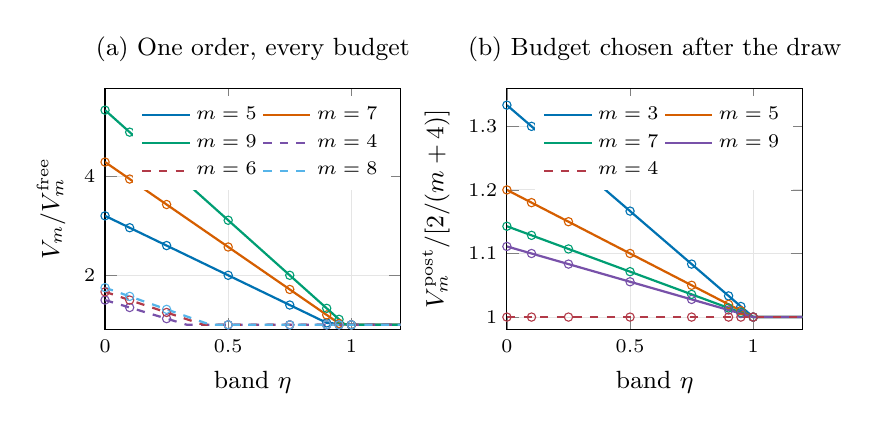
\begin{tikzpicture}
\begin{groupplot}[group style={group size=2 by 1,horizontal sep=1.35cm},width=0.44\textwidth,height=4.65cm,scale only axis=false,tick label style={font=\scriptsize},label style={font=\small},title style={font=\small},legend style={font=\scriptsize,draw=none,fill=white},grid=major,grid style={black!10},/tikz/mark size=1.5pt,unbounded coords=jump]
\nextgroupplot[title={(a) One order, every budget},xlabel={band $\eta$},ylabel={$V_m/V_m^{\rm free}$},xmin=0,xmax=1.2,ymin=0.9,legend columns=2,legend pos=north east]
\addplot+[cblue,no marks,thick] coordinates {(0,3.2) (0.0133333333,3.168) (0.0266666667,3.136) (0.04,3.104) (0.0533333333,3.072) (0.0666666667,3.04) (0.08,3.008) (0.0933333333,2.976) (0.106666667,2.944) (0.12,2.912) (0.133333333,2.88) (0.146666667,2.848) (0.16,2.816) (0.173333333,2.784) (0.186666667,2.752) (0.2,2.72) (0.213333333,2.688) (0.226666667,2.656) (0.24,2.624) (0.253333333,2.592) (0.266666667,2.56) (0.28,2.528) (0.293333333,2.496) (0.306666667,2.464) (0.32,2.432) (0.333333333,2.4) (0.346666667,2.368) (0.36,2.336) (0.373333333,2.304) (0.386666667,2.272) (0.4,2.24) (0.413333333,2.208) (0.426666667,2.176) (0.44,2.144) (0.453333333,2.112) (0.466666667,2.08) (0.48,2.048) (0.493333333,2.016) (0.506666667,1.984) (0.52,1.952) (0.533333333,1.92) (0.546666667,1.888) (0.56,1.856) (0.573333333,1.824) (0.586666667,1.792) (0.6,1.76) (0.613333333,1.728) (0.626666667,1.696) (0.64,1.664) (0.653333333,1.632) (0.666666667,1.6) (0.68,1.568) (0.693333333,1.536) (0.706666667,1.504) (0.72,1.472) (0.733333333,1.44) (0.746666667,1.408) (0.76,1.376) (0.773333333,1.344) (0.786666667,1.312) (0.8,1.28) (0.813333333,1.248) (0.826666667,1.216) (0.84,1.184) (0.853333333,1.152) (0.866666667,1.12) (0.88,1.088) (0.893333333,1.056) (0.9,1.04) (0.906666667,1.03733333) (0.92,1.032) (0.933333333,1.02666667) (0.946666667,1.02133333) (0.96,1.016) (0.973333333,1.01066667) (0.986666667,1.00533333) (1,1) (1.01333333,1) (1.02666667,1) (1.04,1) (1.05333333,1) (1.06666667,1) (1.08,1) (1.09333333,1) (1.10666667,1) (1.12,1) (1.13333333,1) (1.14666667,1) (1.16,1) (1.17333333,1) (1.18666667,1) (1.2,1)};
\addlegendentry{$m=5$}
\addplot+[cblue,only marks,mark=o,forget plot] coordinates {(0,3.2) (0.1,2.96) (0.25,2.6) (0.5,2) (0.75,1.4) (0.9,1.04) (0.95,1.02) (1,1)};
\addplot+[corange,no marks,thick] coordinates {(0,4.28571429) (0.0133333333,4.24) (0.0266666667,4.19428571) (0.04,4.14857143) (0.0533333333,4.10285714) (0.0666666667,4.05714286) (0.08,4.01142857) (0.0933333333,3.96571429) (0.106666667,3.92) (0.12,3.87428571) (0.133333333,3.82857143) (0.146666667,3.78285714) (0.16,3.73714286) (0.173333333,3.69142857) (0.186666667,3.64571429) (0.2,3.6) (0.213333333,3.55428571) (0.226666667,3.50857143) (0.24,3.46285714) (0.253333333,3.41714286) (0.266666667,3.37142857) (0.28,3.32571429) (0.293333333,3.28) (0.306666667,3.23428571) (0.32,3.18857143) (0.333333333,3.14285714) (0.346666667,3.09714286) (0.36,3.05142857) (0.373333333,3.00571429) (0.386666667,2.96) (0.4,2.91428571) (0.413333333,2.86857143) (0.426666667,2.82285714) (0.44,2.77714286) (0.453333333,2.73142857) (0.466666667,2.68571429) (0.48,2.64) (0.493333333,2.59428571) (0.506666667,2.54857143) (0.52,2.50285714) (0.533333333,2.45714286) (0.546666667,2.41142857) (0.56,2.36571429) (0.573333333,2.32) (0.586666667,2.27428571) (0.6,2.22857143) (0.613333333,2.18285714) (0.626666667,2.13714286) (0.64,2.09142857) (0.653333333,2.04571429) (0.666666667,2) (0.68,1.95428571) (0.693333333,1.90857143) (0.706666667,1.86285714) (0.72,1.81714286) (0.733333333,1.77142857) (0.746666667,1.72571429) (0.76,1.68) (0.773333333,1.63428571) (0.786666667,1.58857143) (0.8,1.54285714) (0.813333333,1.49714286) (0.826666667,1.45142857) (0.84,1.40571429) (0.853333333,1.36) (0.866666667,1.31428571) (0.88,1.26857143) (0.893333333,1.22285714) (0.906666667,1.17714286) (0.92,1.13142857) (0.933333333,1.08571429) (0.946666667,1.04) (0.952380952,1.02040816) (0.96,1.01714286) (0.973333333,1.01142857) (0.986666667,1.00571429) (1,1) (1.01333333,1) (1.02666667,1) (1.04,1) (1.05333333,1) (1.06666667,1) (1.08,1) (1.09333333,1) (1.10666667,1) (1.12,1) (1.13333333,1) (1.14666667,1) (1.16,1) (1.17333333,1) (1.18666667,1) (1.2,1)};
\addlegendentry{$m=7$}
\addplot+[corange,only marks,mark=o,forget plot] coordinates {(0,4.28571429) (0.1,3.94285714) (0.25,3.42857143) (0.5,2.57142857) (0.75,1.71428571) (0.9,1.2) (0.95,1.02857143) (1,1)};
\addplot+[cgreen,no marks,thick] coordinates {(0,5.33333333) (0.0133333333,5.27407407) (0.0266666667,5.21481481) (0.04,5.15555556) (0.0533333333,5.0962963) (0.0666666667,5.03703704) (0.08,4.97777778) (0.0933333333,4.91851852) (0.106666667,4.85925926) (0.12,4.8) (0.133333333,4.74074074) (0.146666667,4.68148148) (0.16,4.62222222) (0.173333333,4.56296296) (0.186666667,4.5037037) (0.2,4.44444444) (0.213333333,4.38518519) (0.226666667,4.32592593) (0.24,4.26666667) (0.253333333,4.20740741) (0.266666667,4.14814815) (0.28,4.08888889) (0.293333333,4.02962963) (0.306666667,3.97037037) (0.32,3.91111111) (0.333333333,3.85185185) (0.346666667,3.79259259) (0.36,3.73333333) (0.373333333,3.67407407) (0.386666667,3.61481481) (0.4,3.55555556) (0.413333333,3.4962963) (0.426666667,3.43703704) (0.44,3.37777778) (0.453333333,3.31851852) (0.466666667,3.25925926) (0.48,3.2) (0.493333333,3.14074074) (0.506666667,3.08148148) (0.52,3.02222222) (0.533333333,2.96296296) (0.546666667,2.9037037) (0.56,2.84444444) (0.573333333,2.78518519) (0.586666667,2.72592593) (0.6,2.66666667) (0.613333333,2.60740741) (0.626666667,2.54814815) (0.64,2.48888889) (0.653333333,2.42962963) (0.666666667,2.37037037) (0.68,2.31111111) (0.693333333,2.25185185) (0.706666667,2.19259259) (0.72,2.13333333) (0.733333333,2.07407407) (0.746666667,2.01481481) (0.76,1.95555556) (0.773333333,1.8962963) (0.786666667,1.83703704) (0.8,1.77777778) (0.813333333,1.71851852) (0.826666667,1.65925926) (0.84,1.6) (0.853333333,1.54074074) (0.866666667,1.48148148) (0.88,1.42222222) (0.893333333,1.36296296) (0.906666667,1.3037037) (0.92,1.24444444) (0.933333333,1.18518519) (0.946666667,1.12592593) (0.96,1.06666667) (0.972222222,1.01234568) (0.973333333,1.01185185) (0.986666667,1.00592593) (1,1) (1.01333333,1) (1.02666667,1) (1.04,1) (1.05333333,1) (1.06666667,1) (1.08,1) (1.09333333,1) (1.10666667,1) (1.12,1) (1.13333333,1) (1.14666667,1) (1.16,1) (1.17333333,1) (1.18666667,1) (1.2,1)};
\addlegendentry{$m=9$}
\addplot+[cgreen,only marks,mark=o,forget plot] coordinates {(0,5.33333333) (0.1,4.88888889) (0.25,4.22222222) (0.5,3.11111111) (0.75,2) (0.9,1.33333333) (0.95,1.11111111) (1,1)};
\addplot+[cpurple,no marks,thick,dashed] coordinates {(0,1.5) (0.0133333333,1.48) (0.0266666667,1.46) (0.04,1.44) (0.0533333333,1.42) (0.0666666667,1.4) (0.08,1.38) (0.0933333333,1.36) (0.106666667,1.34) (0.12,1.32) (0.133333333,1.3) (0.146666667,1.28) (0.16,1.26) (0.173333333,1.24) (0.186666667,1.22) (0.2,1.2) (0.213333333,1.18) (0.226666667,1.16) (0.24,1.14) (0.253333333,1.12) (0.266666667,1.1) (0.28,1.08) (0.293333333,1.06) (0.306666667,1.04) (0.32,1.02) (0.333333333,1) (0.346666667,1) (0.36,1) (0.373333333,1) (0.386666667,1) (0.4,1) (0.413333333,1) (0.426666667,1) (0.44,1) (0.453333333,1) (0.466666667,1) (0.48,1) (0.493333333,1) (0.506666667,1) (0.52,1) (0.533333333,1) (0.546666667,1) (0.56,1) (0.573333333,1) (0.586666667,1) (0.6,1) (0.613333333,1) (0.626666667,1) (0.64,1) (0.653333333,1) (0.666666667,1) (0.68,1) (0.693333333,1) (0.706666667,1) (0.72,1) (0.733333333,1) (0.746666667,1) (0.76,1) (0.773333333,1) (0.786666667,1) (0.8,1) (0.813333333,1) (0.826666667,1) (0.84,1) (0.853333333,1) (0.866666667,1) (0.88,1) (0.893333333,1) (0.906666667,1) (0.92,1) (0.933333333,1) (0.946666667,1) (0.96,1) (0.973333333,1) (0.986666667,1) (1,1) (1.01333333,1) (1.02666667,1) (1.04,1) (1.05333333,1) (1.06666667,1) (1.08,1) (1.09333333,1) (1.10666667,1) (1.12,1) (1.13333333,1) (1.14666667,1) (1.16,1) (1.17333333,1) (1.18666667,1) (1.2,1)};
\addlegendentry{$m=4$}
\addplot+[cpurple,only marks,mark=o,forget plot] coordinates {(0,1.5) (0.1,1.35) (0.25,1.125) (0.5,1) (0.75,1) (0.9,1) (0.95,1) (1,1)};
\addplot+[cred,no marks,thick,dashed] coordinates {(0,1.66666667) (0.0133333333,1.64444444) (0.0266666667,1.62222222) (0.04,1.6) (0.0533333333,1.57777778) (0.0666666667,1.55555556) (0.08,1.53333333) (0.0933333333,1.51111111) (0.106666667,1.48888889) (0.12,1.46666667) (0.133333333,1.44444444) (0.146666667,1.42222222) (0.16,1.4) (0.173333333,1.37777778) (0.186666667,1.35555556) (0.2,1.33333333) (0.213333333,1.31111111) (0.226666667,1.28888889) (0.24,1.26666667) (0.253333333,1.24444444) (0.266666667,1.22222222) (0.28,1.2) (0.293333333,1.17777778) (0.306666667,1.15555556) (0.32,1.13333333) (0.333333333,1.11111111) (0.346666667,1.08888889) (0.36,1.06666667) (0.373333333,1.04444444) (0.386666667,1.02222222) (0.4,1) (0.413333333,1) (0.426666667,1) (0.44,1) (0.453333333,1) (0.466666667,1) (0.48,1) (0.493333333,1) (0.506666667,1) (0.52,1) (0.533333333,1) (0.546666667,1) (0.56,1) (0.573333333,1) (0.586666667,1) (0.6,1) (0.613333333,1) (0.626666667,1) (0.64,1) (0.653333333,1) (0.666666667,1) (0.68,1) (0.693333333,1) (0.706666667,1) (0.72,1) (0.733333333,1) (0.746666667,1) (0.76,1) (0.773333333,1) (0.786666667,1) (0.8,1) (0.813333333,1) (0.826666667,1) (0.84,1) (0.853333333,1) (0.866666667,1) (0.88,1) (0.893333333,1) (0.906666667,1) (0.92,1) (0.933333333,1) (0.946666667,1) (0.96,1) (0.973333333,1) (0.986666667,1) (1,1) (1.01333333,1) (1.02666667,1) (1.04,1) (1.05333333,1) (1.06666667,1) (1.08,1) (1.09333333,1) (1.10666667,1) (1.12,1) (1.13333333,1) (1.14666667,1) (1.16,1) (1.17333333,1) (1.18666667,1) (1.2,1)};
\addlegendentry{$m=6$}
\addplot+[cred,only marks,mark=o,forget plot] coordinates {(0,1.66666667) (0.1,1.5) (0.25,1.25) (0.5,1) (0.75,1) (0.9,1) (0.95,1) (1,1)};
\addplot+[cteal,no marks,thick,dashed] coordinates {(0,1.75) (0.0133333333,1.72666667) (0.0266666667,1.70333333) (0.04,1.68) (0.0533333333,1.65666667) (0.0666666667,1.63333333) (0.08,1.61) (0.0933333333,1.58666667) (0.106666667,1.56333333) (0.12,1.54) (0.133333333,1.51666667) (0.146666667,1.49333333) (0.16,1.47) (0.173333333,1.44666667) (0.186666667,1.42333333) (0.2,1.4) (0.213333333,1.37666667) (0.226666667,1.35333333) (0.24,1.33) (0.253333333,1.30666667) (0.266666667,1.28333333) (0.28,1.26) (0.293333333,1.23666667) (0.306666667,1.21333333) (0.32,1.19) (0.333333333,1.16666667) (0.346666667,1.14333333) (0.36,1.12) (0.373333333,1.09666667) (0.386666667,1.07333333) (0.4,1.05) (0.413333333,1.02666667) (0.426666667,1.00333333) (0.428571429,1) (0.44,1) (0.453333333,1) (0.466666667,1) (0.48,1) (0.493333333,1) (0.506666667,1) (0.52,1) (0.533333333,1) (0.546666667,1) (0.56,1) (0.573333333,1) (0.586666667,1) (0.6,1) (0.613333333,1) (0.626666667,1) (0.64,1) (0.653333333,1) (0.666666667,1) (0.68,1) (0.693333333,1) (0.706666667,1) (0.72,1) (0.733333333,1) (0.746666667,1) (0.76,1) (0.773333333,1) (0.786666667,1) (0.8,1) (0.813333333,1) (0.826666667,1) (0.84,1) (0.853333333,1) (0.866666667,1) (0.88,1) (0.893333333,1) (0.906666667,1) (0.92,1) (0.933333333,1) (0.946666667,1) (0.96,1) (0.973333333,1) (0.986666667,1) (1,1) (1.01333333,1) (1.02666667,1) (1.04,1) (1.05333333,1) (1.06666667,1) (1.08,1) (1.09333333,1) (1.10666667,1) (1.12,1) (1.13333333,1) (1.14666667,1) (1.16,1) (1.17333333,1) (1.18666667,1) (1.2,1)};
\addlegendentry{$m=8$}
\addplot+[cteal,only marks,mark=o,forget plot] coordinates {(0,1.75) (0.1,1.575) (0.25,1.3125) (0.5,1) (0.75,1) (0.9,1) (0.95,1) (1,1)};
\nextgroupplot[title={(b) Budget chosen after the draw},xlabel={band $\eta$},ylabel={$V_m^{\rm post}/[2/(m+4)]$},xmin=0,xmax=1.2,ymin=0.98,ymax=1.36,legend columns=2,legend pos=north east]
\addplot+[cblue,no marks,thick] coordinates {(0,1.33333333) (1,1) (1.2,1)};
\addlegendentry{$m=3$}
\addplot+[cblue,only marks,mark=o,forget plot] coordinates {(0,1.33333333) (0.1,1.3) (0.25,1.25) (0.5,1.16666667) (0.75,1.08333333) (0.9,1.03333333) (0.95,1.01666667) (1,1)};
\addplot+[corange,no marks,thick] coordinates {(0,1.2) (1,1) (1.2,1)};
\addlegendentry{$m=5$}
\addplot+[corange,only marks,mark=o,forget plot] coordinates {(0,1.2) (0.1,1.18) (0.25,1.15) (0.5,1.1) (0.75,1.05) (0.9,1.02) (0.95,1.01) (1,1)};
\addplot+[cgreen,no marks,thick] coordinates {(0,1.14285714) (1,1) (1.2,1)};
\addlegendentry{$m=7$}
\addplot+[cgreen,only marks,mark=o,forget plot] coordinates {(0,1.14285714) (0.1,1.12857143) (0.25,1.10714286) (0.5,1.07142857) (0.75,1.03571429) (0.9,1.01428571) (0.95,1.00714286) (1,1)};
\addplot+[cpurple,no marks,thick] coordinates {(0,1.11111111) (1,1) (1.2,1)};
\addlegendentry{$m=9$}
\addplot+[cpurple,only marks,mark=o,forget plot] coordinates {(0,1.11111111) (0.1,1.1) (0.25,1.08333333) (0.5,1.05555556) (0.75,1.02777778) (0.9,1.01111111) (0.95,1.00555556) (1,1)};
\addplot+[cred,no marks,thick,dashed] coordinates {(0,1) (1,1) (1.2,1)};
\addlegendentry{$m=4$}
\addplot+[cred,only marks,mark=o,forget plot] coordinates {(0,1) (0.1,1) (0.25,1) (0.5,1) (0.75,1) (0.9,1) (0.95,1) (1,1)};
\end{groupplot}
\end{tikzpicture}
\caption{The cost of the marginal constraint depends on when the budget is chosen. Lines are Theorems~\ref{thm:even}, \ref{thm:odd} and~\ref{thm:expostband}; circles are stored floating-point LP values (\NUM). In (a), even sizes are dashed and odd sizes solid. Each panel uses its own unconstrained value as denominator: the ex-post denominator is $m-1$ times the ex-ante one. The small band price in (b) therefore does not mean a small absolute loss.}
\label{fig:ctheorems}
\end{figure*}

\begin{figure*}[t]
\centering
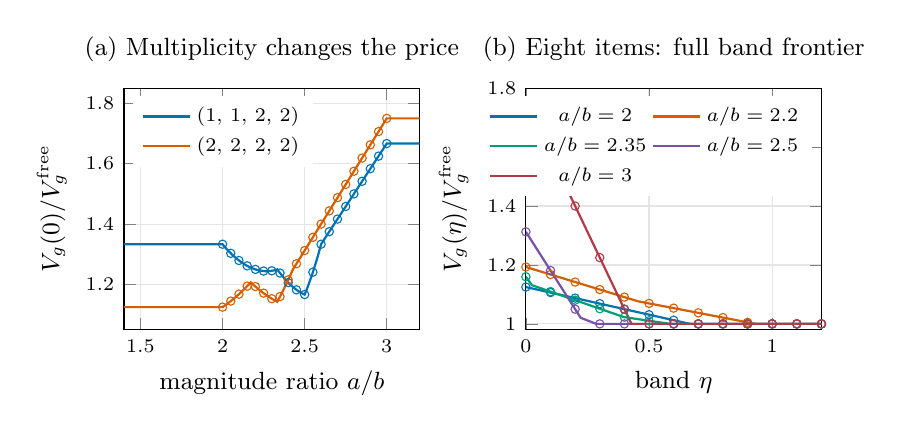
\begin{tikzpicture}
\begin{groupplot}[group style={group size=2 by 1,horizontal sep=1.35cm},width=0.44\textwidth,height=4.65cm,scale only axis=false,tick label style={font=\scriptsize},label style={font=\small},title style={font=\small},legend style={font=\scriptsize,draw=none,fill=white},grid=major,grid style={black!10},/tikz/mark size=1.5pt,unbounded coords=jump]
\nextgroupplot[title={(a) Multiplicity changes the price},xlabel={magnitude ratio $a/b$},ylabel={$V_g(0)/V_g^{\rm free}$},xmin=1.4,xmax=3.2,ymin=1.05,ymax=1.85,legend pos=north west]
\addplot+[cblue,no marks,thick] coordinates {(1.4,1.33333333) (1.409,1.33333333) (1.418,1.33333333) (1.427,1.33333333) (1.436,1.33333333) (1.445,1.33333333) (1.454,1.33333333) (1.463,1.33333333) (1.472,1.33333333) (1.481,1.33333333) (1.49,1.33333333) (1.499,1.33333333) (1.508,1.33333333) (1.517,1.33333333) (1.526,1.33333333) (1.535,1.33333333) (1.544,1.33333333) (1.553,1.33333333) (1.562,1.33333333) (1.571,1.33333333) (1.58,1.33333333) (1.589,1.33333333) (1.598,1.33333333) (1.607,1.33333333) (1.616,1.33333333) (1.625,1.33333333) (1.634,1.33333333) (1.643,1.33333333) (1.652,1.33333333) (1.661,1.33333333) (1.67,1.33333333) (1.679,1.33333333) (1.688,1.33333333) (1.697,1.33333333) (1.706,1.33333333) (1.715,1.33333333) (1.724,1.33333333) (1.733,1.33333333) (1.742,1.33333333) (1.751,1.33333333) (1.76,1.33333333) (1.769,1.33333333) (1.778,1.33333333) (1.787,1.33333333) (1.796,1.33333333) (1.805,1.33333333) (1.814,1.33333333) (1.823,1.33333333) (1.832,1.33333333) (1.841,1.33333333) (1.85,1.33333333) (1.859,1.33333333) (1.868,1.33333333) (1.877,1.33333333) (1.886,1.33333333) (1.895,1.33333333) (1.904,1.33333333) (1.913,1.33333333) (1.922,1.33333333) (1.931,1.33333333) (1.94,1.33333333) (1.949,1.33333333) (1.958,1.33333333) (1.967,1.33333333) (1.976,1.33333333) (1.985,1.33333333) (1.994,1.33333333) (2,1.33333333) (2.003,1.33134532) (2.012,1.32552421) (2.021,1.31991542) (2.03,1.3145164) (2.039,1.30932482) (2.048,1.30433853) (2.057,1.29955559) (2.066,1.29497424) (2.075,1.29059292) (2.084,1.28641024) (2.093,1.28242503) (2.102,1.27863627) (2.111,1.27504314) (2.12,1.27164502) (2.129,1.26844147) (2.138,1.26543222) (2.147,1.26261723) (2.156,1.25999661) (2.165,1.2575707) (2.17157288,1.25592232) (2.174,1.25534001) (2.183,1.25330527) (2.192,1.25146743) (2.201,1.24982762) (2.21,1.24838721) (2.219,1.24714779) (2.228,1.24611118) (2.237,1.24527943) (2.246,1.24465487) (2.255,1.24424004) (2.264,1.24403779) (2.273,1.24405123) (2.282,1.24428375) (2.291,1.24473908) (2.3,1.24542125) (2.309,1.24633461) (2.318,1.24748389) (2.327,1.2488742) (2.33333333,1.25) (2.336,1.24801) (2.345,1.24144177) (2.354,1.23510281) (2.363,1.22899455) (2.372,1.22311873) (2.381,1.2174774) (2.39,1.21207296) (2.399,1.20690815) (2.408,1.20198608) (2.417,1.19731025) (2.426,1.19288459) (2.42857143,1.19166667) (2.435,1.18871347) (2.444,1.18480174) (2.453,1.18115475) (2.462,1.1777784) (2.471,1.17467917) (2.48,1.17186417) (2.489,1.1693412) (2.498,1.1671188) (2.5,1.16666667) (2.507,1.17613252) (2.516,1.18870523) (2.525,1.20175439) (2.534,1.21530758) (2.543,1.2293946) (2.552,1.24404762) (2.561,1.25930144) (2.57,1.2751938) (2.579,1.29176564) (2.588,1.30906149) (2.597,1.32712986) (2.6,1.33333333) (2.606,1.33833333) (2.615,1.34583333) (2.624,1.35333333) (2.633,1.36083333) (2.642,1.36833333) (2.651,1.37583333) (2.66,1.38333333) (2.669,1.39083333) (2.678,1.39833333) (2.687,1.40583333) (2.696,1.41333333) (2.705,1.42083333) (2.714,1.42833333) (2.723,1.43583333) (2.732,1.44333333) (2.741,1.45083333) (2.75,1.45833333) (2.759,1.46583333) (2.768,1.47333333) (2.777,1.48083333) (2.786,1.48833333) (2.795,1.49583333) (2.804,1.50333333) (2.813,1.51083333) (2.822,1.51833333) (2.831,1.52583333) (2.84,1.53333333) (2.849,1.54083333) (2.858,1.54833333) (2.867,1.55583333) (2.876,1.56333333) (2.885,1.57083333) (2.894,1.57833333) (2.903,1.58583333) (2.912,1.59333333) (2.921,1.60083333) (2.93,1.60833333) (2.939,1.61583333) (2.948,1.62333333) (2.957,1.63083333) (2.966,1.63833333) (2.975,1.64583333) (2.984,1.65333333) (2.993,1.66083333) (3,1.66666667) (3.002,1.66666667) (3.011,1.66666667) (3.02,1.66666667) (3.029,1.66666667) (3.038,1.66666667) (3.047,1.66666667) (3.056,1.66666667) (3.065,1.66666667) (3.074,1.66666667) (3.083,1.66666667) (3.092,1.66666667) (3.101,1.66666667) (3.11,1.66666667) (3.119,1.66666667) (3.128,1.66666667) (3.137,1.66666667) (3.146,1.66666667) (3.155,1.66666667) (3.164,1.66666667) (3.173,1.66666667) (3.182,1.66666667) (3.191,1.66666667) (3.2,1.66666667)};
\addlegendentry{(1, 1, 2, 2)}
\addplot+[cblue,only marks,mark=o,forget plot] coordinates {(2,1.33333333) (2.05,1.30325815) (2.1,1.27946128) (2.15,1.26172208) (2.2,1.25) (2.25,1.24444444) (2.3,1.24542125) (2.35,1.23789174) (2.4,1.20634921) (2.45,1.18234065) (2.5,1.16666667) (2.55,1.24074074) (2.6,1.33333333) (2.65,1.375) (2.7,1.41666667) (2.75,1.45833333) (2.8,1.5) (2.85,1.54166667) (2.9,1.58333333) (2.95,1.625) (3,1.66666667)};
\addplot+[corange,no marks,thick] coordinates {(1.4,1.125) (1.409,1.125) (1.418,1.125) (1.427,1.125) (1.436,1.125) (1.445,1.125) (1.454,1.125) (1.463,1.125) (1.472,1.125) (1.481,1.125) (1.49,1.125) (1.499,1.125) (1.508,1.125) (1.517,1.125) (1.526,1.125) (1.535,1.125) (1.544,1.125) (1.553,1.125) (1.562,1.125) (1.571,1.125) (1.58,1.125) (1.589,1.125) (1.598,1.125) (1.607,1.125) (1.616,1.125) (1.625,1.125) (1.634,1.125) (1.643,1.125) (1.652,1.125) (1.661,1.125) (1.67,1.125) (1.679,1.125) (1.688,1.125) (1.697,1.125) (1.706,1.125) (1.715,1.125) (1.724,1.125) (1.733,1.125) (1.742,1.125) (1.751,1.125) (1.76,1.125) (1.769,1.125) (1.778,1.125) (1.787,1.125) (1.796,1.125) (1.805,1.125) (1.814,1.125) (1.823,1.125) (1.832,1.125) (1.841,1.125) (1.85,1.125) (1.859,1.125) (1.868,1.125) (1.877,1.125) (1.886,1.125) (1.895,1.125) (1.904,1.125) (1.913,1.125) (1.922,1.125) (1.931,1.125) (1.94,1.125) (1.949,1.125) (1.958,1.125) (1.967,1.125) (1.976,1.125) (1.985,1.125) (1.994,1.125) (2,1.125) (2.003,1.12612951) (2.012,1.12957287) (2.021,1.13310023) (2.03,1.13671392) (2.039,1.14041636) (2.048,1.14421008) (2.057,1.14809769) (2.066,1.15208191) (2.075,1.15616554) (2.084,1.16035153) (2.093,1.16464292) (2.102,1.16904287) (2.111,1.1735547) (2.12,1.17818182) (2.129,1.18292781) (2.138,1.1877964) (2.147,1.19279147) (2.156,1.19791706) (2.165,1.2031774) (2.17157288,1.20710678) (2.174,1.20587713) (2.183,1.20138346) (2.192,1.19699447) (2.201,1.19271114) (2.21,1.18853457) (2.219,1.18446592) (2.228,1.18050646) (2.237,1.17665757) (2.246,1.17292074) (2.255,1.16929753) (2.264,1.16578968) (2.273,1.16239899) (2.282,1.15912745) (2.291,1.15597714) (2.3,1.15295031) (2.309,1.15004937) (2.318,1.14727689) (2.327,1.1446356) (2.33333333,1.14285714) (2.336,1.14555826) (2.345,1.15478361) (2.354,1.16418335) (2.363,1.17376585) (2.372,1.18353992) (2.381,1.19351486) (2.39,1.20370053) (2.399,1.21410734) (2.408,1.22474634) (2.417,1.23562924) (2.426,1.24676846) (2.42857143,1.25) (2.435,1.255625) (2.444,1.2635) (2.453,1.271375) (2.462,1.27925) (2.471,1.287125) (2.48,1.295) (2.489,1.302875) (2.498,1.31075) (2.5,1.3125) (2.507,1.318625) (2.516,1.3265) (2.525,1.334375) (2.534,1.34225) (2.543,1.350125) (2.552,1.358) (2.561,1.365875) (2.57,1.37375) (2.579,1.381625) (2.588,1.3895) (2.597,1.397375) (2.6,1.4) (2.606,1.40525) (2.615,1.413125) (2.624,1.421) (2.633,1.428875) (2.642,1.43675) (2.651,1.444625) (2.66,1.4525) (2.669,1.460375) (2.678,1.46825) (2.687,1.476125) (2.696,1.484) (2.705,1.491875) (2.714,1.49975) (2.723,1.507625) (2.732,1.5155) (2.741,1.523375) (2.75,1.53125) (2.759,1.539125) (2.768,1.547) (2.777,1.554875) (2.786,1.56275) (2.795,1.570625) (2.804,1.5785) (2.813,1.586375) (2.822,1.59425) (2.831,1.602125) (2.84,1.61) (2.849,1.617875) (2.858,1.62575) (2.867,1.633625) (2.876,1.6415) (2.885,1.649375) (2.894,1.65725) (2.903,1.665125) (2.912,1.673) (2.921,1.680875) (2.93,1.68875) (2.939,1.696625) (2.948,1.7045) (2.957,1.712375) (2.966,1.72025) (2.975,1.728125) (2.984,1.736) (2.993,1.743875) (3,1.75) (3.002,1.75) (3.011,1.75) (3.02,1.75) (3.029,1.75) (3.038,1.75) (3.047,1.75) (3.056,1.75) (3.065,1.75) (3.074,1.75) (3.083,1.75) (3.092,1.75) (3.101,1.75) (3.11,1.75) (3.119,1.75) (3.128,1.75) (3.137,1.75) (3.146,1.75) (3.155,1.75) (3.164,1.75) (3.173,1.75) (3.182,1.75) (3.191,1.75) (3.2,1.75)};
\addlegendentry{(2, 2, 2, 2)}
\addplot+[corange,only marks,mark=o,forget plot] coordinates {(2,1.125) (2.05,1.14506579) (2.1,1.16805556) (2.15,1.19448529) (2.2,1.19318182) (2.25,1.1712963) (2.3,1.15295031) (2.35,1.15998363) (2.4,1.21527778) (2.45,1.26875) (2.5,1.3125) (2.55,1.35625) (2.6,1.4) (2.65,1.44375) (2.7,1.4875) (2.75,1.53125) (2.8,1.575) (2.85,1.61875) (2.9,1.6625) (2.95,1.70625) (3,1.75)};
\nextgroupplot[title={(b) Eight items: full band frontier},xlabel={band $\eta$},ylabel={$V_g(\eta)/V_g^{\rm free}$},xmin=0,xmax=1.2,ymin=0.98,ymax=1.8,legend columns=2,legend pos=north east]
\addplot+[cblue,no marks,thick] coordinates {(0,1.125) (0.012,1.12275) (0.024,1.1205) (0.036,1.11825) (0.048,1.116) (0.06,1.11375) (0.072,1.1115) (0.084,1.10925) (0.096,1.107) (0.108,1.10475) (0.12,1.1025) (0.132,1.10025) (0.144,1.098) (0.156,1.09575) (0.168,1.0935) (0.18,1.09125) (0.192,1.089) (0.204,1.08675) (0.216,1.0845) (0.228,1.08225) (0.24,1.08) (0.252,1.07775) (0.264,1.0755) (0.276,1.07325) (0.288,1.071) (0.3,1.06875) (0.312,1.0665) (0.324,1.06425) (0.336,1.062) (0.348,1.05975) (0.36,1.0575) (0.372,1.05525) (0.384,1.053) (0.396,1.05075) (0.408,1.0485) (0.42,1.04625) (0.432,1.044) (0.444,1.04175) (0.456,1.0395) (0.468,1.03725) (0.48,1.035) (0.492,1.03275) (0.504,1.0305) (0.516,1.02825) (0.528,1.026) (0.54,1.02375) (0.552,1.0215) (0.564,1.01925) (0.576,1.017) (0.588,1.01475) (0.6,1.0125) (0.612,1.01025) (0.624,1.008) (0.636,1.00575) (0.648,1.0035) (0.66,1.00125) (0.666666667,1) (0.672,1) (0.684,1) (0.696,1) (0.708,1) (0.72,1) (0.732,1) (0.744,1) (0.756,1) (0.768,1) (0.78,1) (0.792,1) (0.804,1) (0.816,1) (0.828,1) (0.84,1) (0.852,1) (0.864,1) (0.876,1) (0.888,1) (0.9,1) (0.912,1) (0.924,1) (0.936,1) (0.948,1) (0.96,1) (0.972,1) (0.984,1) (0.996,1) (1.008,1) (1.02,1) (1.032,1) (1.044,1) (1.056,1) (1.068,1) (1.08,1) (1.092,1) (1.104,1) (1.116,1) (1.128,1) (1.14,1) (1.152,1) (1.164,1) (1.176,1) (1.188,1) (1.2,1)};
\addlegendentry{$a/b=2$}
\addplot+[cblue,only marks,mark=o,forget plot] coordinates {(0,1.125) (0.1,1.10625) (0.2,1.0875) (0.3,1.06875) (0.4,1.05) (0.5,1.03125) (0.6,1.0125) (0.7,1) (0.8,1) (0.9,1) (1,1) (1.1,1) (1.2,1)};
\addplot+[corange,no marks,thick] coordinates {(0,1.19318182) (0.012,1.19011364) (0.0222222222,1.1875) (0.024,1.18704545) (0.036,1.18397727) (0.048,1.18090909) (0.06,1.17784091) (0.072,1.17477273) (0.084,1.17170455) (0.096,1.16863636) (0.108,1.16556818) (0.12,1.1625) (0.132,1.15943182) (0.144,1.15636364) (0.156,1.15329545) (0.168,1.15022727) (0.18,1.14715909) (0.192,1.14409091) (0.204,1.14102273) (0.216,1.13795455) (0.228,1.13488636) (0.24,1.13181818) (0.252,1.12875) (0.264,1.12568182) (0.276,1.12261364) (0.288,1.11954545) (0.3,1.11647727) (0.312,1.11340909) (0.324,1.11034091) (0.336,1.10727273) (0.348,1.10420455) (0.36,1.10113636) (0.372,1.09806818) (0.384,1.095) (0.396,1.09193182) (0.408,1.08886364) (0.42,1.08579545) (0.432,1.08272727) (0.444,1.07965909) (0.456,1.07659091) (0.456140351,1.07655502) (0.468,1.07465241) (0.48,1.07272727) (0.492,1.07080214) (0.504,1.06887701) (0.516,1.06695187) (0.528,1.06502674) (0.54,1.0631016) (0.552,1.06117647) (0.564,1.05925134) (0.576,1.0573262) (0.588,1.05540107) (0.6,1.05347594) (0.612,1.0515508) (0.624,1.04962567) (0.636,1.04770053) (0.648,1.0457754) (0.66,1.04385027) (0.672,1.04192513) (0.684,1.04) (0.696,1.03807487) (0.708,1.03614973) (0.72,1.0342246) (0.732,1.03229947) (0.744,1.03037433) (0.755555556,1.0285205) (0.756,1.0284492) (0.768,1.02652406) (0.78,1.02459893) (0.792,1.0226738) (0.804,1.02074866) (0.816,1.01882353) (0.828,1.0168984) (0.84,1.01497326) (0.852,1.01304813) (0.864,1.01112299) (0.876,1.00919786) (0.888,1.00727273) (0.9,1.00534759) (0.912,1.00342246) (0.924,1.00149733) (0.933333333,1) (0.936,1) (0.948,1) (0.96,1) (0.972,1) (0.984,1) (0.996,1) (1.008,1) (1.02,1) (1.032,1) (1.044,1) (1.056,1) (1.068,1) (1.08,1) (1.092,1) (1.104,1) (1.116,1) (1.128,1) (1.14,1) (1.152,1) (1.164,1) (1.176,1) (1.188,1) (1.2,1)};
\addlegendentry{$a/b=2.2$}
\addplot+[corange,only marks,mark=o,forget plot] coordinates {(0,1.19318182) (0.1,1.16761364) (0.2,1.14204545) (0.3,1.11647727) (0.4,1.09090909) (0.5,1.06951872) (0.6,1.05347594) (0.7,1.03743316) (0.8,1.02139037) (0.9,1.00534759) (1,1) (1.1,1) (1.2,1)};
\addplot+[cgreen,no marks,thick] coordinates {(0,1.15998363) (0.012,1.14606383) (0.024,1.13214403) (0.024691358,1.13134206) (0.036,1.1280626) (0.048,1.12458265) (0.06,1.1211027) (0.072,1.11762275) (0.084,1.1141428) (0.0847118186,1.11393637) (0.096,1.11066285) (0.108,1.1071829) (0.12,1.10370295) (0.132,1.100223) (0.137918871,1.09850655) (0.144,1.09674304) (0.156,1.09326309) (0.168,1.08978314) (0.18,1.08630319) (0.192,1.08282324) (0.204,1.07934329) (0.216,1.07586334) (0.228,1.07238339) (0.24,1.06890344) (0.252,1.06542349) (0.264,1.06194354) (0.276,1.05846358) (0.288,1.05498363) (0.3,1.05150368) (0.312,1.04802373) (0.324,1.04454378) (0.336,1.04106383) (0.348,1.03758388) (0.36,1.03410393) (0.372,1.03062398) (0.384,1.02714403) (0.396,1.02366408) (0.397512016,1.0232256) (0.408,1.02193493) (0.42,1.02045819) (0.432,1.01898145) (0.444,1.01750471) (0.456,1.01602797) (0.468,1.01455123) (0.477601411,1.01336966) (0.48,1.01307449) (0.492,1.01159775) (0.504,1.01012101) (0.516,1.00864427) (0.528,1.00716753) (0.54,1.00569079) (0.552,1.00421405) (0.564,1.00273731) (0.576,1.00126057) (0.586243386,1) (0.588,1) (0.6,1) (0.612,1) (0.624,1) (0.636,1) (0.648,1) (0.66,1) (0.672,1) (0.684,1) (0.696,1) (0.708,1) (0.72,1) (0.732,1) (0.744,1) (0.756,1) (0.768,1) (0.78,1) (0.792,1) (0.804,1) (0.816,1) (0.828,1) (0.84,1) (0.852,1) (0.864,1) (0.876,1) (0.888,1) (0.9,1) (0.912,1) (0.924,1) (0.936,1) (0.948,1) (0.96,1) (0.972,1) (0.984,1) (0.996,1) (1.008,1) (1.02,1) (1.032,1) (1.044,1) (1.056,1) (1.068,1) (1.08,1) (1.092,1) (1.104,1) (1.116,1) (1.128,1) (1.14,1) (1.152,1) (1.164,1) (1.176,1) (1.188,1) (1.2,1)};
\addlegendentry{$a/b=2.35$}
\addplot+[cgreen,only marks,mark=o,forget plot] coordinates {(0,1.15998363) (0.1,1.10950286) (0.2,1.08050327) (0.3,1.05150368) (0.4,1.02291942) (0.5,1.01061325) (0.6,1) (0.7,1) (0.8,1) (0.9,1) (1,1) (1.1,1) (1.2,1)};
\addplot+[cpurple,no marks,thick] coordinates {(0,1.3125) (0.012,1.29675) (0.024,1.281) (0.036,1.26525) (0.048,1.2495) (0.06,1.23375) (0.072,1.218) (0.084,1.20225) (0.096,1.1865) (0.108,1.17075) (0.12,1.155) (0.132,1.13925) (0.144,1.1235) (0.156,1.10775) (0.168,1.092) (0.18,1.07625) (0.192,1.0605) (0.204,1.04475) (0.216,1.029) (0.222222222,1.02083333) (0.228,1.0189375) (0.238095238,1.015625) (0.24,1.015) (0.252,1.0110625) (0.264,1.007125) (0.276,1.0031875) (0.285714286,1) (0.288,1) (0.3,1) (0.312,1) (0.324,1) (0.336,1) (0.348,1) (0.36,1) (0.372,1) (0.384,1) (0.396,1) (0.408,1) (0.42,1) (0.432,1) (0.444,1) (0.456,1) (0.468,1) (0.48,1) (0.492,1) (0.504,1) (0.516,1) (0.528,1) (0.54,1) (0.552,1) (0.564,1) (0.576,1) (0.588,1) (0.6,1) (0.612,1) (0.624,1) (0.636,1) (0.648,1) (0.66,1) (0.672,1) (0.684,1) (0.696,1) (0.708,1) (0.72,1) (0.732,1) (0.744,1) (0.756,1) (0.768,1) (0.78,1) (0.792,1) (0.804,1) (0.816,1) (0.828,1) (0.84,1) (0.852,1) (0.864,1) (0.876,1) (0.888,1) (0.9,1) (0.912,1) (0.924,1) (0.936,1) (0.948,1) (0.96,1) (0.972,1) (0.984,1) (0.996,1) (1.008,1) (1.02,1) (1.032,1) (1.044,1) (1.056,1) (1.068,1) (1.08,1) (1.092,1) (1.104,1) (1.116,1) (1.128,1) (1.14,1) (1.152,1) (1.164,1) (1.176,1) (1.188,1) (1.2,1)};
\addlegendentry{$a/b=2.5$}
\addplot+[cpurple,only marks,mark=o,forget plot] coordinates {(0,1.3125) (0.1,1.18125) (0.2,1.05) (0.3,1) (0.4,1) (0.5,1) (0.6,1) (0.7,1) (0.8,1) (0.9,1) (1,1) (1.1,1) (1.2,1)};
\addplot+[cred,no marks,thick] coordinates {(0,1.75) (0.012,1.729) (0.024,1.708) (0.036,1.687) (0.048,1.666) (0.06,1.645) (0.072,1.624) (0.084,1.603) (0.096,1.582) (0.108,1.561) (0.12,1.54) (0.132,1.519) (0.144,1.498) (0.156,1.477) (0.168,1.456) (0.18,1.435) (0.192,1.414) (0.204,1.393) (0.216,1.372) (0.228,1.351) (0.24,1.33) (0.252,1.309) (0.264,1.288) (0.276,1.267) (0.288,1.246) (0.3,1.225) (0.312,1.204) (0.324,1.183) (0.336,1.162) (0.348,1.141) (0.36,1.12) (0.372,1.099) (0.384,1.078) (0.396,1.057) (0.408,1.036) (0.42,1.015) (0.428571429,1) (0.432,1) (0.444,1) (0.456,1) (0.468,1) (0.48,1) (0.492,1) (0.504,1) (0.516,1) (0.528,1) (0.54,1) (0.552,1) (0.564,1) (0.576,1) (0.588,1) (0.6,1) (0.612,1) (0.624,1) (0.636,1) (0.648,1) (0.66,1) (0.666666667,1) (0.672,1) (0.684,1) (0.696,1) (0.708,1) (0.72,1) (0.732,1) (0.744,1) (0.756,1) (0.768,1) (0.78,1) (0.792,1) (0.804,1) (0.816,1) (0.828,1) (0.84,1) (0.852,1) (0.864,1) (0.876,1) (0.888,1) (0.9,1) (0.912,1) (0.924,1) (0.936,1) (0.948,1) (0.96,1) (0.972,1) (0.984,1) (0.996,1) (1.008,1) (1.02,1) (1.032,1) (1.044,1) (1.056,1) (1.068,1) (1.08,1) (1.092,1) (1.104,1) (1.116,1) (1.128,1) (1.14,1) (1.152,1) (1.164,1) (1.176,1) (1.188,1) (1.2,1)};
\addlegendentry{$a/b=3$}
\addplot+[cred,only marks,mark=o,forget plot] coordinates {(0,1.75) (0.1,1.575) (0.2,1.4) (0.3,1.225) (0.4,1.05) (0.5,1) (0.6,1) (0.7,1) (0.8,1) (0.9,1) (1,1) (1.1,1) (1.2,1)};
\end{groupplot}
\end{tikzpicture}
\caption{Beyond the parity family. Exact curves from Theorems~\ref{thm:twomagprice}, \ref{thm:twomag1122} and~\ref{thm:twomag2222}; circles are the pre-existing ratio-refinement LP results. Both count patterns have even size, yet their prices are nonmonotone in $a/b$ and their active constraints change. In (b), all curves are proved for every band; sampled markers only check the transcription of the formulas.}
\label{fig:chetero}
\end{figure*}

\begin{figure*}[t]
\centering
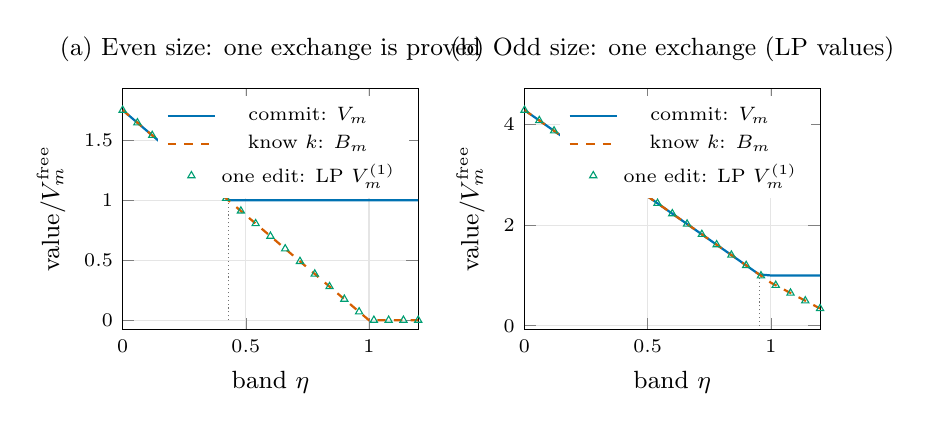
\begin{tikzpicture}
\begin{groupplot}[group style={group size=2 by 1,horizontal sep=1.35cm},width=0.44\textwidth,height=4.65cm,scale only axis=false,tick label style={font=\scriptsize},label style={font=\small},title style={font=\small},legend style={font=\scriptsize,draw=none,fill=white},grid=major,grid style={black!10},/tikz/mark size=1.5pt,unbounded coords=jump]
\nextgroupplot[title={(a) Even size: one exchange is proved},xlabel={band $\eta$},ylabel={value$/V_m^{\rm free}$},xmin=0,xmax=1.2,ymin=-0.08,legend pos=north east]
\addplot+[cblue,no marks,thick] coordinates {(0,1.75) (0.0109090909,1.73090909) (0.0218181818,1.71181818) (0.0327272727,1.69272727) (0.0436363636,1.67363636) (0.0545454545,1.65454545) (0.0654545455,1.63545455) (0.0763636364,1.61636364) (0.0872727273,1.59727273) (0.0981818182,1.57818182) (0.109090909,1.55909091) (0.12,1.54) (0.130909091,1.52090909) (0.141818182,1.50181818) (0.152727273,1.48272727) (0.163636364,1.46363636) (0.174545455,1.44454545) (0.185454545,1.42545455) (0.196363636,1.40636364) (0.207272727,1.38727273) (0.218181818,1.36818182) (0.229090909,1.34909091) (0.24,1.33) (0.250909091,1.31090909) (0.261818182,1.29181818) (0.272727273,1.27272727) (0.283636364,1.25363636) (0.294545455,1.23454545) (0.305454545,1.21545455) (0.316363636,1.19636364) (0.327272727,1.17727273) (0.338181818,1.15818182) (0.349090909,1.13909091) (0.36,1.12) (0.370909091,1.10090909) (0.381818182,1.08181818) (0.392727273,1.06272727) (0.403636364,1.04363636) (0.414545455,1.02454545) (0.425454545,1.00545455) (0.428571429,1) (0.436363636,1) (0.447272727,1) (0.458181818,1) (0.469090909,1) (0.48,1) (0.490909091,1) (0.501818182,1) (0.512727273,1) (0.523636364,1) (0.534545455,1) (0.545454545,1) (0.556363636,1) (0.567272727,1) (0.578181818,1) (0.589090909,1) (0.6,1) (0.610909091,1) (0.621818182,1) (0.632727273,1) (0.643636364,1) (0.654545455,1) (0.665454545,1) (0.676363636,1) (0.687272727,1) (0.698181818,1) (0.709090909,1) (0.72,1) (0.730909091,1) (0.741818182,1) (0.752727273,1) (0.763636364,1) (0.774545455,1) (0.785454545,1) (0.796363636,1) (0.807272727,1) (0.818181818,1) (0.829090909,1) (0.84,1) (0.850909091,1) (0.861818182,1) (0.872727273,1) (0.883636364,1) (0.894545455,1) (0.905454545,1) (0.916363636,1) (0.927272727,1) (0.938181818,1) (0.949090909,1) (0.96,1) (0.970909091,1) (0.981818182,1) (0.992727273,1) (1,1) (1.00363636,1) (1.01454545,1) (1.02545455,1) (1.03636364,1) (1.04727273,1) (1.05818182,1) (1.06909091,1) (1.08,1) (1.09090909,1) (1.10181818,1) (1.11272727,1) (1.12363636,1) (1.13454545,1) (1.14545455,1) (1.15636364,1) (1.16727273,1) (1.17818182,1) (1.18909091,1) (1.2,1)};
\addlegendentry{commit: $V_m$}
\addplot+[corange,no marks,thick,dashed] coordinates {(0,1.75) (0.0109090909,1.73090909) (0.0218181818,1.71181818) (0.0327272727,1.69272727) (0.0436363636,1.67363636) (0.0545454545,1.65454545) (0.0654545455,1.63545455) (0.0763636364,1.61636364) (0.0872727273,1.59727273) (0.0981818182,1.57818182) (0.109090909,1.55909091) (0.12,1.54) (0.130909091,1.52090909) (0.141818182,1.50181818) (0.152727273,1.48272727) (0.163636364,1.46363636) (0.174545455,1.44454545) (0.185454545,1.42545455) (0.196363636,1.40636364) (0.207272727,1.38727273) (0.218181818,1.36818182) (0.229090909,1.34909091) (0.24,1.33) (0.250909091,1.31090909) (0.261818182,1.29181818) (0.272727273,1.27272727) (0.283636364,1.25363636) (0.294545455,1.23454545) (0.305454545,1.21545455) (0.316363636,1.19636364) (0.327272727,1.17727273) (0.338181818,1.15818182) (0.349090909,1.13909091) (0.36,1.12) (0.370909091,1.10090909) (0.381818182,1.08181818) (0.392727273,1.06272727) (0.403636364,1.04363636) (0.414545455,1.02454545) (0.425454545,1.00545455) (0.428571429,1) (0.436363636,0.986363636) (0.447272727,0.967272727) (0.458181818,0.948181818) (0.469090909,0.929090909) (0.48,0.91) (0.490909091,0.890909091) (0.501818182,0.871818182) (0.512727273,0.852727273) (0.523636364,0.833636364) (0.534545455,0.814545455) (0.545454545,0.795454545) (0.556363636,0.776363636) (0.567272727,0.757272727) (0.578181818,0.738181818) (0.589090909,0.719090909) (0.6,0.7) (0.610909091,0.680909091) (0.621818182,0.661818182) (0.632727273,0.642727273) (0.643636364,0.623636364) (0.654545455,0.604545455) (0.665454545,0.585454545) (0.676363636,0.566363636) (0.687272727,0.547272727) (0.698181818,0.528181818) (0.709090909,0.509090909) (0.72,0.49) (0.730909091,0.470909091) (0.741818182,0.451818182) (0.752727273,0.432727273) (0.763636364,0.413636364) (0.774545455,0.394545455) (0.785454545,0.375454545) (0.796363636,0.356363636) (0.807272727,0.337272727) (0.818181818,0.318181818) (0.829090909,0.299090909) (0.84,0.28) (0.850909091,0.260909091) (0.861818182,0.241818182) (0.872727273,0.222727273) (0.883636364,0.203636364) (0.894545455,0.184545455) (0.905454545,0.165454545) (0.916363636,0.146363636) (0.927272727,0.127272727) (0.938181818,0.108181818) (0.949090909,0.0890909091) (0.96,0.07) (0.970909091,0.0509090909) (0.981818182,0.0318181818) (0.992727273,0.0127272727) (1,0) (1.00363636,0) (1.01454545,0) (1.02545455,0) (1.03636364,0) (1.04727273,0) (1.05818182,0) (1.06909091,0) (1.08,0) (1.09090909,0) (1.10181818,0) (1.11272727,0) (1.12363636,0) (1.13454545,0) (1.14545455,0) (1.15636364,0) (1.16727273,0) (1.17818182,0) (1.18909091,0) (1.2,0)};
\addlegendentry{know $k$: $B_m$}
\addplot+[cgreen,only marks,mark=triangle] coordinates {(0,1.75) (0.06,1.645) (0.12,1.54) (0.18,1.435) (0.24,1.33) (0.3,1.225) (0.36,1.12) (0.42,1.015) (0.48,0.91) (0.54,0.805) (0.6,0.7) (0.66,0.595) (0.72,0.49) (0.78,0.385) (0.84,0.28) (0.9,0.175) (0.96,0.07) (1.02,0) (1.08,0) (1.14,0) (1.2,0)};
\addlegendentry{one edit: LP $V^{(1)}_m$}
\addplot+[black!55,no marks,densely dotted,forget plot] coordinates {(0.428571429,0) (0.428571429,1)};
\nextgroupplot[title={(b) Odd size: one exchange (LP values)},xlabel={band $\eta$},ylabel={value$/V_m^{\rm free}$},xmin=0,xmax=1.2,ymin=-0.08,legend pos=north east]
\addplot+[cblue,no marks,thick] coordinates {(0,4.28571429) (0.0109090909,4.24831169) (0.0218181818,4.21090909) (0.0327272727,4.17350649) (0.0436363636,4.1361039) (0.0545454545,4.0987013) (0.0654545455,4.0612987) (0.0763636364,4.0238961) (0.0872727273,3.98649351) (0.0981818182,3.94909091) (0.109090909,3.91168831) (0.12,3.87428571) (0.130909091,3.83688312) (0.141818182,3.79948052) (0.152727273,3.76207792) (0.163636364,3.72467532) (0.174545455,3.68727273) (0.185454545,3.64987013) (0.196363636,3.61246753) (0.207272727,3.57506494) (0.218181818,3.53766234) (0.229090909,3.50025974) (0.24,3.46285714) (0.250909091,3.42545455) (0.261818182,3.38805195) (0.272727273,3.35064935) (0.283636364,3.31324675) (0.294545455,3.27584416) (0.305454545,3.23844156) (0.316363636,3.20103896) (0.327272727,3.16363636) (0.338181818,3.12623377) (0.349090909,3.08883117) (0.36,3.05142857) (0.370909091,3.01402597) (0.381818182,2.97662338) (0.392727273,2.93922078) (0.403636364,2.90181818) (0.414545455,2.86441558) (0.425454545,2.82701299) (0.436363636,2.78961039) (0.447272727,2.75220779) (0.458181818,2.71480519) (0.469090909,2.6774026) (0.48,2.64) (0.490909091,2.6025974) (0.501818182,2.56519481) (0.512727273,2.52779221) (0.523636364,2.49038961) (0.534545455,2.45298701) (0.545454545,2.41558442) (0.556363636,2.37818182) (0.567272727,2.34077922) (0.578181818,2.30337662) (0.589090909,2.26597403) (0.6,2.22857143) (0.610909091,2.19116883) (0.621818182,2.15376623) (0.632727273,2.11636364) (0.643636364,2.07896104) (0.654545455,2.04155844) (0.665454545,2.00415584) (0.676363636,1.96675325) (0.687272727,1.92935065) (0.698181818,1.89194805) (0.709090909,1.85454545) (0.72,1.81714286) (0.730909091,1.77974026) (0.741818182,1.74233766) (0.752727273,1.70493506) (0.763636364,1.66753247) (0.774545455,1.63012987) (0.785454545,1.59272727) (0.796363636,1.55532468) (0.807272727,1.51792208) (0.818181818,1.48051948) (0.829090909,1.44311688) (0.84,1.40571429) (0.850909091,1.36831169) (0.861818182,1.33090909) (0.872727273,1.29350649) (0.883636364,1.2561039) (0.894545455,1.2187013) (0.905454545,1.1812987) (0.916363636,1.1438961) (0.927272727,1.10649351) (0.938181818,1.06909091) (0.949090909,1.03168831) (0.952380952,1.02040816) (0.96,1.01714286) (0.970909091,1.01246753) (0.981818182,1.00779221) (0.992727273,1.00311688) (1,1) (1.00363636,1) (1.01454545,1) (1.02545455,1) (1.03636364,1) (1.04727273,1) (1.05818182,1) (1.06909091,1) (1.08,1) (1.09090909,1) (1.10181818,1) (1.11272727,1) (1.12363636,1) (1.13454545,1) (1.14545455,1) (1.15636364,1) (1.16727273,1) (1.17818182,1) (1.18909091,1) (1.2,1)};
\addlegendentry{commit: $V_m$}
\addplot+[corange,no marks,thick,dashed] coordinates {(0,4.28571429) (0.0109090909,4.24831169) (0.0218181818,4.21090909) (0.0327272727,4.17350649) (0.0436363636,4.1361039) (0.0545454545,4.0987013) (0.0654545455,4.0612987) (0.0763636364,4.0238961) (0.0872727273,3.98649351) (0.0981818182,3.94909091) (0.109090909,3.91168831) (0.12,3.87428571) (0.130909091,3.83688312) (0.141818182,3.79948052) (0.152727273,3.76207792) (0.163636364,3.72467532) (0.174545455,3.68727273) (0.185454545,3.64987013) (0.196363636,3.61246753) (0.207272727,3.57506494) (0.218181818,3.53766234) (0.229090909,3.50025974) (0.24,3.46285714) (0.250909091,3.42545455) (0.261818182,3.38805195) (0.272727273,3.35064935) (0.283636364,3.31324675) (0.294545455,3.27584416) (0.305454545,3.23844156) (0.316363636,3.20103896) (0.327272727,3.16363636) (0.338181818,3.12623377) (0.349090909,3.08883117) (0.36,3.05142857) (0.370909091,3.01402597) (0.381818182,2.97662338) (0.392727273,2.93922078) (0.403636364,2.90181818) (0.414545455,2.86441558) (0.425454545,2.82701299) (0.436363636,2.78961039) (0.447272727,2.75220779) (0.458181818,2.71480519) (0.469090909,2.6774026) (0.48,2.64) (0.490909091,2.6025974) (0.501818182,2.56519481) (0.512727273,2.52779221) (0.523636364,2.49038961) (0.534545455,2.45298701) (0.545454545,2.41558442) (0.556363636,2.37818182) (0.567272727,2.34077922) (0.578181818,2.30337662) (0.589090909,2.26597403) (0.6,2.22857143) (0.610909091,2.19116883) (0.621818182,2.15376623) (0.632727273,2.11636364) (0.643636364,2.07896104) (0.654545455,2.04155844) (0.665454545,2.00415584) (0.676363636,1.96675325) (0.687272727,1.92935065) (0.698181818,1.89194805) (0.709090909,1.85454545) (0.72,1.81714286) (0.730909091,1.77974026) (0.741818182,1.74233766) (0.752727273,1.70493506) (0.763636364,1.66753247) (0.774545455,1.63012987) (0.785454545,1.59272727) (0.796363636,1.55532468) (0.807272727,1.51792208) (0.818181818,1.48051948) (0.829090909,1.44311688) (0.84,1.40571429) (0.850909091,1.36831169) (0.861818182,1.33090909) (0.872727273,1.29350649) (0.883636364,1.2561039) (0.894545455,1.2187013) (0.905454545,1.1812987) (0.916363636,1.1438961) (0.927272727,1.10649351) (0.938181818,1.06909091) (0.949090909,1.03168831) (0.952380952,1.02040816) (0.96,0.994285714) (0.970909091,0.956883117) (0.981818182,0.919480519) (0.992727273,0.882077922) (1,0.857142857) (1.00363636,0.847792208) (1.01454545,0.81974026) (1.02545455,0.791688312) (1.03636364,0.763636364) (1.04727273,0.735584416) (1.05818182,0.707532468) (1.06909091,0.679480519) (1.08,0.651428571) (1.09090909,0.623376623) (1.10181818,0.595324675) (1.11272727,0.567272727) (1.12363636,0.539220779) (1.13454545,0.511168831) (1.14545455,0.483116883) (1.15636364,0.455064935) (1.16727273,0.427012987) (1.17818182,0.398961039) (1.18909091,0.370909091) (1.2,0.342857143)};
\addlegendentry{know $k$: $B_m$}
\addplot+[cgreen,only marks,mark=triangle] coordinates {(0,4.28571429) (0.06,4.08) (0.12,3.87428571) (0.18,3.66857143) (0.24,3.46285714) (0.3,3.25714286) (0.36,3.05142857) (0.42,2.84571429) (0.48,2.64) (0.54,2.43428571) (0.6,2.22857143) (0.66,2.02285714) (0.72,1.81714286) (0.78,1.61142857) (0.84,1.40571429) (0.9,1.2) (0.96,0.994285714) (1.02,0.805714286) (1.08,0.651428571) (1.14,0.497142857) (1.2,0.342857143)};
\addlegendentry{one edit: LP $V^{(1)}_m$}
\addplot+[black!55,no marks,densely dotted,forget plot] coordinates {(0.952380952,0) (0.952380952,1.02040816)};
\end{groupplot}
\end{tikzpicture}
\caption{When commitment costs something, and what one edit recovers. Here $m=8$ (left) and $m=7$ (right). Solid and dashed curves are the proved universal and budget-aware values; the dotted vertical line is the exact onset of a positive gap. Triangles are saved one-exchange LP values. Their equality to $B_m$ is proved for every size and band: even sizes by Theorem~\ref{thm:awareexact}, odd sizes by \lean{recourse\_one\_odd\_all} (formalized after these LP runs); the triangles remain the saved LP values. Both the initial and edited laws obey the marginal band.}
\label{fig:crecourse}
\end{figure*}

\begin{figure*}[t]
\centering
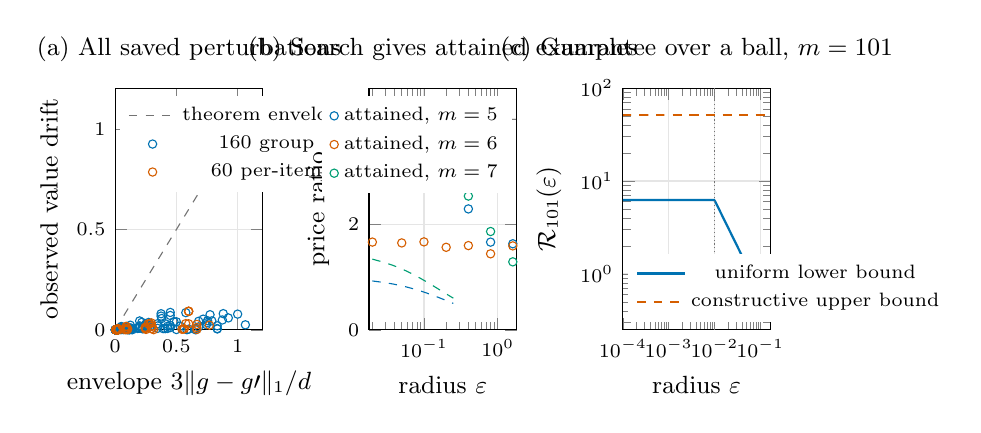
\begin{tikzpicture}
\begin{groupplot}[group style={group size=3 by 1,horizontal sep=1.35cm},width=0.285\textwidth,height=4.65cm,scale only axis=false,tick label style={font=\scriptsize},label style={font=\small},title style={font=\small},legend style={font=\scriptsize,draw=none,fill=white},grid=major,grid style={black!10},/tikz/mark size=1.5pt,unbounded coords=jump]
\nextgroupplot[title={(a) All saved perturbations},xlabel={envelope $3\Vert g-g\prime\Vert_1/d$},ylabel={observed value drift},xmin=0,ymin=0,legend pos=north west]
\addplot+[black!55,no marks,dashed] coordinates {(0,0) (1.09512514,1.09512514)};
\addlegendentry{theorem envelope}
\addplot+[cblue,only marks,mark=o] coordinates {(0.00333333333,0.000199679463) (0.01,0.000824110037) (0.0267428373,0.00484842505) (0.0666666667,0.0075780745) (0.133333333,0.00342558813) (0.266666667,0.0246851037) (0.6,0.00296938081) (0.833333333,0.00607578683) (0.00333704116,7.75564886e-05) (0.0100061756,0.000173117075) (0.0267663544,0.00391389061) (0.0666666667,0.00186905363) (0.133333333,0.00804563736) (0.266666667,0.0157172647) (0.5,0.0399944828) (1.06322829,0.0248952302) (0.00333333333,0.000107426552) (0.0100235114,0.000945848711) (0.0266666667,0.00191977044) (0.0666666667,0.00421320211) (0.133333333,0.00372779553) (0.273931997,0.0367518702) (0.530301802,0.0186222726) (0.833333333,0.0197579413) (0.00333653805,9.59238643e-05) (0.01,0.000391589685) (0.0268567708,0.00254593321) (0.0681309011,0.00117614368) (0.138869981,2.86971846e-05) (0.290891134,0.0205461915) (0.5,0.00132627166) (0.88257919,0.0805205419) (0.00300111616,0.000512194773) (0.009,0.00168728872) (0.0241070081,0.00138774174) (0.06,0.0127928778) (0.12,0.000966080919) (0.250408489,0.028621871) (0.45,0.0713955839) (0.875229644,0.0489909911) (0.003,7.73196522e-06) (0.009,0.0013086003) (0.0241935484,0.00329496194) (0.06,0.00232217817) (0.124231859,0.0227778444) (0.258541738,0.023561801) (0.45,0.0865145947) (1,0.0781122895) (0.003,3.59898066e-05) (0.009,0.000651001854) (0.024,0.00177784131) (0.0601244674,0.00728277682) (0.125,0.00342328951) (0.246230691,0.00961833867) (0.479608083,0.0406847982) (0.75,0.0356147356) (0.003,0.000222687489) (0.0090158355,0.000752810564) (0.024,0.00233057341) (0.06,0.00387548061) (0.12,0.00120287676) (0.252980923,0.0214767686) (0.45,0.0219352837) (0.923964185,0.0591796104) (0.00272833224,5.60194149e-05) (0.00819505727,0.00161133756) (0.021854552,0.00371134578) (0.0546429235,0.0123600995) (0.112680956,0.000479708969) (0.226302037,0.00468200709) (0.409090909,0.00590259604) (0.745465342,0.0253579752) (0.00272727273,0.000235099133) (0.00818397623,0.00052677724) (0.0218181818,0.000711477987) (0.0545454545,0.00282365036) (0.109090909,0.0119995615) (0.218181818,0.0371518416) (0.451066286,0.0114251984) (0.8343941,0.00428964881) (0.00272825377,6.43917693e-05) (0.00820106844,4.91490329e-05) (0.021978022,0.00114483966) (0.0545454545,0.00361815629) (0.113207547,0.000770245542) (0.22208726,0.0133074831) (0.409090909,0.0303291216) (0.681818182,0.0143671256) (0.00272802771,2.64473056e-05) (0.00819859005,0.000102490929) (0.021958931,0.00114878435) (0.055433569,0.00477464951) (0.109090909,0.00913065518) (0.218181818,0.00731132419) (0.42808069,0.00675559844) (0.681818182,0.0425929311) (0.00250208507,0.000235315756) (0.00751460797,0.0015137061) (0.0200835149,5.11288982e-05) (0.0502958644,0.0162166153) (0.1,0.000597557613) (0.2,0.0147665317) (0.375,0.0800927746) (0.789473684,0.0445294443) (0.00250024998,0.000558624826) (0.0075,0.000488967187) (0.02,0.00174650686) (0.05,0.00323014004) (0.102141509,0.0130372752) (0.2,0.0441329238) (0.375,0.0681952937) (0.75451189,0.0452156941) (0.0025,0.000154929028) (0.0075,0.000543346231) (0.02,0.00154134376) (0.05,0.00732347396) (0.102028041,0.0124182205) (0.2,0.0081987399) (0.379953315,0.0561101103) (0.718349861,0.053059212) (0.0025,4.3720708e-05) (0.00751201119,0.000267801251) (0.0200327049,0.00123082638) (0.0507598073,0.001439586) (0.1,0.00338895379) (0.201005497,0.0195919502) (0.428571429,0.017727299) (0.7746348,0.0752316116) (0.00230769231,0.000362733222) (0.00692307692,0.00137496322) (0.0184750979,0.0013031454) (0.0464309468,0.00458803993) (0.0925713886,0.00524487809) (0.184615385,0.0112465107) (0.346153846,0.0189953415) (0.576923077,0.0855364688) (0.00230769231,0.000494139359) (0.00692307692,4.17603269e-05) (0.0184615385,0.00110316823) (0.0466166462,0.00726164514) (0.0923076923,0.00136896343) (0.184615385,0.00748555925) (0.346153846,0.00730180922) (0.657950576,0.00622986007) (0.00230769231,0.000125844485) (0.00692307692,0.000462024155) (0.0184615385,0.00119813981) (0.0466208546,0.00329276278) (0.0923076923,0.00548929747) (0.184615385,0.00704497364) (0.391304348,0.0060457855) (0.585378837,0.000339229842) (0.00230769231,0.000199317663) (0.00692307692,0.00033805365) (0.0184615385,0.000548957826) (0.0461538462,0.00131261238) (0.0923076923,0.00354772331) (0.187700169,0.0112114645) (0.346153846,0.0303003496) (0.657133252,2.56091712e-05)};
\addlegendentry{160 group}
\addplot+[corange,only marks,mark=o] coordinates {(0.00666666667,0.000204192448) (0.0266666667,0.00018309772) (0.100389582,0.00408365977) (0.314261812,0.000674447488) (0.666666667,0.0268739048) (0.00666666667,5.84306719e-05) (0.0266666667,0.000309522905) (0.101797333,0.00409128175) (0.3,0.017071523) (0.666666667,0.00162520384) (0.00667112212,0.000581917977) (0.0268079603,0.000114423755) (0.10085043,0.00404265562) (0.3,0.0192280886) (0.666666667,0.0116849798) (0.00667365935,0.000741517518) (0.0266666667,0.00117744333) (0.100659055,0.000511500765) (0.3,0.00596424458) (0.76940089,0.0232818985) (0.006,0.000325702087) (0.0241079235,0.00285959831) (0.0902992038,0.017313834) (0.284864753,0.0298032171) (0.6,0.0922204786) (0.00600118461,0.0011649136) (0.0240295063,0.00654014545) (0.0903722927,0.0153625291) (0.295169011,0.0344006709) (0.6,0.0915843916) (0.006,0.000438083071) (0.0240604404,0.00152115256) (0.09,0.00506395315) (0.27,0.0298003551) (0.6,0.0927809045) (0.006,0.000313224426) (0.024,0.00125890017) (0.09,0.00429996632) (0.295688817,0.00627950409) (0.6,0.0299184282) (0.00545454545,0.000668051141) (0.0218181818,0.00143478704) (0.0822957897,0.00550502505) (0.247257708,0.0083019549) (0.557309478,0.00421573659) (0.00545454545,0.00021044757) (0.0218181818,0.000185505372) (0.0818181818,0.000736120954) (0.245640253,0.00593290065) (0.545454545,0.00270318699) (0.00545655116,0.000218229671) (0.0218909996,0.00129886278) (0.0818181818,0.00330222616) (0.245454545,0.0122824645) (0.564957316,0.00441951989) (0.00546063263,0.000174070989) (0.0218181818,0.000387371106) (0.0818181818,0.00138000547) (0.252343267,0.00182214385) (0.576563147,0.0307448491)};
\addlegendentry{60 per-item}
\nextgroupplot[title={(b) Search gives attained examples},xlabel={radius $\varepsilon$},ylabel={price ratio},xmode=log,xmin=0.018,xmax=1.8,ymin=0,legend pos=north east]
\addplot+[cblue,only marks,mark=o] coordinates {(0.02,3.1396117) (0.05,3.05922572) (0.1,2.92018956) (0.2,2.68901864) (0.4,2.29144036) (0.8,1.66184503) (1.6,1.63056516)};
\addlegendentry{attained, $m=5$}
\addplot+[cblue,no marks,dashed,forget plot] coordinates {(0.02,0.925925926) (0.0292,0.895415473) (0.0384,0.866851595) (0.0476,0.840053763) (0.0568,0.814863103) (0.066,0.791139241) (0.0752,0.768757688) (0.0844,0.747607656) (0.0936,0.727590221) (0.1028,0.70861678) (0.112,0.690607735) (0.1212,0.673491379) (0.1304,0.657202944) (0.1396,0.641683778) (0.1488,0.626880642) (0.158,0.612745098) (0.1672,0.599232982) (0.1764,0.58630394) (0.1856,0.573921028) (0.1948,0.56205036) (0.204,0.550660793) (0.2132,0.539723661) (0.2224,0.529212532) (0.2316,0.51910299) (0.2408,0.509372453) (0.25,0.5)};
\addplot+[corange,only marks,mark=o] coordinates {(0.02,1.66256601) (0.05,1.64684115) (0.1,1.66666667) (0.2,1.56368006) (0.4,1.59644238) (0.8,1.44045085) (1.6,1.59051964)};
\addlegendentry{attained, $m=6$}
\addplot+[cgreen,only marks,mark=o] coordinates {(0.02,4.1635627) (0.05,3.99136) (0.1,3.72466539) (0.2,3.27715354) (0.4,2.53506837) (0.8,1.86316269) (1.6,1.28799804)};
\addlegendentry{attained, $m=7$}
\addplot+[cgreen,no marks,dashed,forget plot] coordinates {(0.02,1.33928571) (0.0292,1.27637849) (0.0384,1.21911573) (0.0476,1.16677038) (0.0568,1.11873508) (0.066,1.07449857) (0.0752,1.03362734) (0.0844,0.99575146) (0.0936,0.960553279) (0.1028,0.927758535) (0.112,0.897129187) (0.1212,0.868457619) (0.1304,0.841561939) (0.1396,0.816282107) (0.1488,0.792476754) (0.158,0.770020534) (0.1672,0.748801917) (0.1764,0.728721337) (0.1856,0.709689629) (0.1948,0.691626706) (0.204,0.674460432) (0.2132,0.658125658) (0.2224,0.6425634) (0.2316,0.627720121) (0.2408,0.61354712) (0.25,0.6)};
\nextgroupplot[title={(c) Guarantee over a ball, $m=101$},xlabel={radius $\varepsilon$},ylabel={$\mathcal R_{101}(\varepsilon)$},xmode=log,ymode=log,xmin=0.0001,xmax=0.167,ymin=0.25,ymax=100,legend pos=south west]
\addplot+[cblue,no marks,thick] coordinates {(0.0001,6.25) (0.000104745785,6.25) (0.000109716794,6.25) (0.000114923717,6.25) (0.000120377749,6.25) (0.000126090618,6.25) (0.000132074607,6.25) (0.000138342584,6.25) (0.000144908025,6.25) (0.000151785048,6.25) (0.00015898844,6.25) (0.000166533689,6.25) (0.000174437019,6.25) (0.000182715424,6.25) (0.000191386705,6.25) (0.000200469506,6.25) (0.000209983357,6.25) (0.000219948715,6.25) (0.000230387008,6.25) (0.000241320679,6.25) (0.000252773239,6.25) (0.000264769313,6.25) (0.000277334694,6.25) (0.000290496402,6.25) (0.000304282736,6.25) (0.000318723339,6.25) (0.000333849263,6.25) (0.00034969303,6.25) (0.000366288709,6.25) (0.000383671982,6.25) (0.000401880229,6.25) (0.000420952599,6.25) (0.000440930103,6.25) (0.000461855697,6.25) (0.000483774374,6.25) (0.000506733264,6.25) (0.000530781734,6.25) (0.000555971492,6.25) (0.000582356702,6.25) (0.000609994098,6.25) (0.000638943104,6.25) (0.000669265968,6.25) (0.00070102789,6.25) (0.000734297165,6.25) (0.000769145328,6.25) (0.000805647309,6.25) (0.000843881596,6.25) (0.0008839304,6.25) (0.000925879834,6.25) (0.000969820097,6.25) (0.00101584567,6.25) (0.00106405552,6.25) (0.0011145533,6.25) (0.0011674476,6.25) (0.00122285215,6.25) (0.00128088608,6.25) (0.00134167418,6.25) (0.00140534715,6.25) (0.0014720419,6.25) (0.00154190184,6.25) (0.00161507718,6.25) (0.00169172527,6.25) (0.00177201091,6.25) (0.00185610673,6.25) (0.00194419356,6.25) (0.0020364608,6.25) (0.00213310684,6.25) (0.0022343395,6.25) (0.00234037645,6.25) (0.00245144567,6.25) (0.00256778601,6.25) (0.0026896476,6.25) (0.00281729249,6.25) (0.00295099512,6.25) (0.003091043,6.25) (0.00323773725,6.25) (0.00339139329,6.25) (0.00355234151,6.25) (0.00372092799,6.25) (0.00389751522,6.25) (0.0040824829,6.25) (0.00427622875,6.25) (0.00447916937,6.25) (0.0046917411,6.25) (0.00491440103,6.25) (0.00514762793,6.25) (0.00539192326,6.25) (0.00564781234,6.25) (0.00591584535,6.25) (0.00619659863,6.25) (0.00649067587,6.25) (0.00679870937,6.25) (0.00712136148,6.25) (0.00745932596,6.25) (0.00781332952,6.25) (0.00818413331,6.25) (0.00857253466,6.25) (0.0089793687,6.25) (0.00940551021,6.25) (0.00985187547,6.25) (0.0103194243,6.05653943) (0.0108091619,5.7821319) (0.0113221415,5.52015712) (0.011859466,5.27005181) (0.0124222907,5.03127818) (0.0130118258,4.80332282) (0.0136293391,4.58569558) (0.0142761582,4.37792852) (0.0149536739,4.17957489) (0.0156633431,3.9902082) (0.0164066916,3.80942127) (0.0171853179,3.63682536) (0.0180008961,3.47204938) (0.0188551799,3.314739) (0.0197500061,3.16455598) (0.0206872989,3.02117741) (0.0216690735,2.88429498) (0.0226974411,2.75361437) (0.0237746128,2.62885459) (0.0249029048,2.50974738) (0.026084743,2.39603664) (0.0273226687,2.28747787) (0.0286193438,2.18383763) (0.0299775562,2.0848931) (0.0314002265,1.9904315) (0.0328904137,1.90024974) (0.0344513219,1.8141539) (0.0360863075,1.73195886) (0.0377988859,1.65348789) (0.0395927397,1.57857225) (0.0414717259,1.50705086) (0.0434398847,1.43876993) (0.0455014481,1.37358266) (0.0476608489,1.31134886) (0.0499227301,1.25193474) (0.0522919554,1.19521252) (0.0547736191,1.14106026) (0.0573730571,1.08936151) (0.0600958589,1.0400051) (0.062947879,0.992884923) (0.0659352498,0.947899647) (0.0690643948,0.904952547) (0.0723420423,0.863951279) (0.0757752399,0.824807682) (0.0793713697,0.78743759) (0.083138164,0.751760648) (0.0870837223,0.717700144) (0.0912165282,0.685182841) (0.0955454683,0.654138821) (0.100079851,0.624501332) (0.104829425,0.596206648) (0.109804404,0.56919393) (0.115015484,0.543405094) (0.120473871,0.518784689) (0.126191302,0.495279777) (0.13218007,0.472839818) (0.138453051,0.45141656) (0.145023735,0.430963939) (0.151906249,0.411437978) (0.159115393,0.392796693) (0.166666667,0.375)};
\addlegendentry{uniform lower bound}
\addplot+[corange,no marks,thick,dashed] coordinates {(0.0001,51.4851485) (0.000104745785,51.4851485) (0.000109716794,51.4851485) (0.000114923717,51.4851485) (0.000120377749,51.4851485) (0.000126090618,51.4851485) (0.000132074607,51.4851485) (0.000138342584,51.4851485) (0.000144908025,51.4851485) (0.000151785048,51.4851485) (0.00015898844,51.4851485) (0.000166533689,51.4851485) (0.000174437019,51.4851485) (0.000182715424,51.4851485) (0.000191386705,51.4851485) (0.000200469506,51.4851485) (0.000209983357,51.4851485) (0.000219948715,51.4851485) (0.000230387008,51.4851485) (0.000241320679,51.4851485) (0.000252773239,51.4851485) (0.000264769313,51.4851485) (0.000277334694,51.4851485) (0.000290496402,51.4851485) (0.000304282736,51.4851485) (0.000318723339,51.4851485) (0.000333849263,51.4851485) (0.00034969303,51.4851485) (0.000366288709,51.4851485) (0.000383671982,51.4851485) (0.000401880229,51.4851485) (0.000420952599,51.4851485) (0.000440930103,51.4851485) (0.000461855697,51.4851485) (0.000483774374,51.4851485) (0.000506733264,51.4851485) (0.000530781734,51.4851485) (0.000555971492,51.4851485) (0.000582356702,51.4851485) (0.000609994098,51.4851485) (0.000638943104,51.4851485) (0.000669265968,51.4851485) (0.00070102789,51.4851485) (0.000734297165,51.4851485) (0.000769145328,51.4851485) (0.000805647309,51.4851485) (0.000843881596,51.4851485) (0.0008839304,51.4851485) (0.000925879834,51.4851485) (0.000969820097,51.4851485) (0.00101584567,51.4851485) (0.00106405552,51.4851485) (0.0011145533,51.4851485) (0.0011674476,51.4851485) (0.00122285215,51.4851485) (0.00128088608,51.4851485) (0.00134167418,51.4851485) (0.00140534715,51.4851485) (0.0014720419,51.4851485) (0.00154190184,51.4851485) (0.00161507718,51.4851485) (0.00169172527,51.4851485) (0.00177201091,51.4851485) (0.00185610673,51.4851485) (0.00194419356,51.4851485) (0.0020364608,51.4851485) (0.00213310684,51.4851485) (0.0022343395,51.4851485) (0.00234037645,51.4851485) (0.00245144567,51.4851485) (0.00256778601,51.4851485) (0.0026896476,51.4851485) (0.00281729249,51.4851485) (0.00295099512,51.4851485) (0.003091043,51.4851485) (0.00323773725,51.4851485) (0.00339139329,51.4851485) (0.00355234151,51.4851485) (0.00372092799,51.4851485) (0.00389751522,51.4851485) (0.0040824829,51.4851485) (0.00427622875,51.4851485) (0.00447916937,51.4851485) (0.0046917411,51.4851485) (0.00491440103,51.4851485) (0.00514762793,51.4851485) (0.00539192326,51.4851485) (0.00564781234,51.4851485) (0.00591584535,51.4851485) (0.00619659863,51.4851485) (0.00649067587,51.4851485) (0.00679870937,51.4851485) (0.00712136148,51.4851485) (0.00745932596,51.4851485) (0.00781332952,51.4851485) (0.00818413331,51.4851485) (0.00857253466,51.4851485) (0.0089793687,51.4851485) (0.00940551021,51.4851485) (0.00985187547,51.4851485) (0.0103194243,51.4851485) (0.0108091619,51.4851485) (0.0113221415,51.4851485) (0.011859466,51.4851485) (0.0124222907,51.4851485) (0.0130118258,51.4851485) (0.0136293391,51.4851485) (0.0142761582,51.4851485) (0.0149536739,51.4851485) (0.0156633431,51.4851485) (0.0164066916,51.4851485) (0.0171853179,51.4851485) (0.0180008961,51.4851485) (0.0188551799,51.4851485) (0.0197500061,51.4851485) (0.0206872989,51.4851485) (0.0216690735,51.4851485) (0.0226974411,51.4851485) (0.0237746128,51.4851485) (0.0249029048,51.4851485) (0.026084743,51.4851485) (0.0273226687,51.4851485) (0.0286193438,51.4851485) (0.0299775562,51.4851485) (0.0314002265,51.4851485) (0.0328904137,51.4851485) (0.0344513219,51.4851485) (0.0360863075,51.4851485) (0.0377988859,51.4851485) (0.0395927397,51.4851485) (0.0414717259,51.4851485) (0.0434398847,51.4851485) (0.0455014481,51.4851485) (0.0476608489,51.4851485) (0.0499227301,51.4851485) (0.0522919554,51.4851485) (0.0547736191,51.4851485) (0.0573730571,51.4851485) (0.0600958589,51.4851485) (0.062947879,51.4851485) (0.0659352498,51.4851485) (0.0690643948,51.4851485) (0.0723420423,51.4851485) (0.0757752399,51.4851485) (0.0793713697,51.4851485) (0.083138164,51.4851485) (0.0870837223,51.4851485) (0.0912165282,51.4851485) (0.0955454683,51.4851485) (0.100079851,51.4851485) (0.104829425,51.4851485) (0.109804404,51.4851485) (0.115015484,51.4851485) (0.120473871,51.4851485) (0.126191302,51.4851485) (0.13218007,51.4851485) (0.138453051,51.4851485) (0.145023735,51.4851485) (0.151906249,51.4851485) (0.159115393,51.4851485) (0.166666667,51.4851485)};
\addlegendentry{constructive upper bound}
\addplot+[black!55,no marks,densely dotted,forget plot] coordinates {(0.0099009901,0.25) (0.0099009901,100)};
\end{groupplot}
\end{tikzpicture}
\caption{Robustness with the quantifiers kept explicit. (a) All 220 saved perturbations, with recomputed baselines and moving normalisation, lie under the envelope; $d=\min(\Vert g\Vert_1,\Vert g\prime\Vert_1)$ and the largest drift/envelope ratio is 0.322. The producer could skip failures; the full prescribed row counts were checked, with none missing. (b) Search returns attained ratios, hence upper bounds on the infimum over the searched ball, not global minimisers. Dashed floors for odd sizes are shown only in their domain $\varepsilon\le1/4$. (c) The two bounds in Corollary~\ref{cor:robustball}, drawn only on $0<\varepsilon\le1/6$; these are theorem bounds, not measured worst-case optima. The vertical line marks $1/m$.}
\label{fig:cstab}
\end{figure*}

% END PAPER C INLINE FIGURES

\section{Limitations}
\label{sec:limits}

\begin{enumerate}
\item[1)] \textbf{Closed forms for $g_m$ and four two-magnitude count patterns.} Closed forms
are proved for $g_{m}$ of~\eqref{eq:family} and, on two magnitudes, for the count patterns
below. Other weights enter through Theorems~\ref{thm:robust}, \ref{thm:collapse},
\ref{thm:typedflow} and~\ref{thm:freeband}, which give an exact program and threshold but no
closed form. On two magnitudes the frontier is proved for one item of each
type (Theorem~\ref{thm:twomag}) and for counts $(2,2,1,1)$ (Theorem~\ref{thm:twomag2211}); for
counts $(1,1,2,2)$ and $(2,2,2,2)$ the whole frontier is exact (Theorems~\ref{thm:twomag1122}
and~\ref{thm:twomag2222}); for other counts the map is floating point on a grid. The physical
interpretation uses the shared binary support in~\eqref{eq:physicalmodel}, not arbitrary
compression architectures.
\item[2)] \textbf{Robustness is a guarantee over a ball.} Corollary~\ref{cor:robustball}
determines the smallest attainable ratio only up to absolute constants and excludes zero
free values. It does not characterise every perturbation, nor give an exact robustness curve.
The exact frontiers at $g_m$ and this perturbation law are different results.
\item[3)] \textbf{Value, not algorithm.} Theorem~\ref{thm:typedflow} gives a program with
at most $\prod_\tau(n_\tau+1)$ count states, polynomial only for a fixed number of types. A generic
perturbation makes every weight distinct, and then $d=m$.
\item[4)] \textbf{Two objectives, kept apart.} Every ex-ante statement concerns
$\max_{k}\mathbb{E}r_{k}$, and every ex-post one concerns $\mathbb{E}\max_{k}r_{k}$.
\item[5)] \textbf{Budget information and recourse.} The value of knowing the budget is exact on
$g_m$ at every band (Theorem~\ref{thm:awareexact}) and on four items at every band
(Theorem~\ref{thm:fourrecourse}). One exchange reaches $B$ at every band on four items and on $g_m$
in every size $m\ge3$: even sizes as stated above, odd sizes by \lean{recourse\_one\_odd\_all} in
\lean{LeanPaperCBudgetExchangeOddV2} (every $\eta\ge0$; formalized after the earlier numerical runs at
$m=5,7,9$, which it subsumes). On the counts $(1,1,2,2)$ and $(2,2,2,2)$ the one-exchange property is
observed numerically at the five tested ratios only; beyond $g_m$ and four items the general
one-exchange statement remains open. Recourse allows one budget reveal and one bounded revision, not a
dynamically changing budget stream.
\end{enumerate}

\section{Conclusion}

For one distribution over orders serving all removal budgets, on the family $g_m$ uniform item
marginals have an exact price that depends sharply on parity. On two magnitudes the exact price
and free threshold depend on the magnitude ratio as well as on the counts. The complete frontier and explicit attaining
laws show where this price disappears; the composition flow preserves the optimisation over
all orders rather than restricting it to a constructed menu. Two changes of quantifier have
different effects. Choosing the budget after the draw raises the free cost but makes the
marginal band almost free. Requiring a guarantee over perturbed weights preserves a linear
odd-size price only to radius of order $1/m$; the guaranteed price thereafter scales as
$1/\varepsilon$ for $\varepsilon\le1/6$, although individual perturbations can preserve the original ratio.
Knowing the budget in advance can be worth nothing: on the family, over a range of bands, one
budget alone forces the universal value. Once the band is loose enough, commitment has a price,
and on four items, and on the family in even size, a single exchange after the budget is
revealed recovers all of it.
These results separate marginal fairness, budget timing and robustness within one precisely
specified compression objective.

\section*{Companion material}
The supplement gives the full proof architecture of each theorem, every supporting Lean
declaration, and the frozen builds it was checked in. The claim map records, for each
headline, its model, its declaration, its scope and its evidence. Corrections made during
preparation are recorded in the project ledger, not in this text.

\begin{thebibliography}{00}

\bibitem{singh2018} A. Singh and T. Joachims, ``Fairness of exposure in rankings,'' in
\emph{Proc. 24th ACM SIGKDD Int. Conf. Knowledge Discovery and Data Mining}, 2018,
pp.~2219--2228.

\bibitem{celis2018} L. E. Celis, D. Straszak, and N. K. Vishnoi, ``Ranking with fairness
constraints,'' in \emph{Proc. 45th Int. Colloq. Automata, Languages, and Programming
(ICALP)}, 2018.

\bibitem{singh2021} A. Singh, D. Kempe, and T. Joachims, ``Fairness in ranking under
uncertainty,'' in \emph{Advances in Neural Information Processing Systems 34}, 2021,
pp.~11896--11908.

\bibitem{disser2023} Y. Disser, M. Klimm, K. Schewior, and D. Weckbecker, ``Incremental
maximization via continuization,'' in \emph{Proc. 50th Int. Colloq. Automata, Languages, and
Programming (ICALP)}, LIPIcs vol.~261, 2023, art.~47.

\bibitem{bienkowski2026} M. Bienkowski, J. Blikstad, J. Byrka, M. Costa, Y. Disser, and
A. Lutz, ``Incremental submodular maximization: Better than greedy,'' arXiv:2606.28558, 2026.

\bibitem{koike2022} T. Koike, L. Lin, and R. Wang, ``Joint mixability and notions of negative
dependence,'' arXiv:2204.11438, 2022.

\bibitem{freeman2020} R. Freeman, N. Shah, and R. Vaish, ``Best of both worlds: Ex-ante and
ex-post fairness in resource allocation,'' in \emph{Proc. 21st ACM Conf. Economics and
Computation (EC)}, 2020.

\bibitem{gupta2022} A. Gupta, V. Gurunathan, R. Krishnaswamy, A. Kumar, and S. Singla,
``Online discrepancy with recourse for vectors and graphs,'' in \emph{Proc. ACM-SIAM Symp.
Discrete Algorithms (SODA)}, 2022.

\bibitem{schrijver2003} A. Schrijver, \emph{Combinatorial Optimization: Polyhedra and
Efficiency}. Berlin, Germany: Springer, 2003.

\bibitem{mathlib2020} The mathlib Community, ``The Lean mathematical library,'' in
\emph{Proc. 9th ACM SIGPLAN Int. Conf. Certified Programs and Proofs (CPP)}, 2020,
pp.~367--381.

\bibitem{demoura2021} L. de Moura and S. Ullrich, ``The Lean 4 theorem prover and
programming language,'' in \emph{Proc. 28th Int. Conf. Automated Deduction (CADE)}, 2021,
pp.~625--635.


\bibitem{storandt2019} S. Storandt and S. Funke, ``Algorithms for average regret minimization,''
in \emph{Proc. AAAI Conf. Artificial Intelligence}, vol.~33, 2019, pp.~1600--1607,
doi: 10.1609/aaai.v33i01.33011600.

\bibitem{bellini2016} F. Bellini, O. E. Kara\c{s}an, and M. \c{C}. P\i nar,
``Joint mixability of some integer matrices,'' \emph{Discrete Optimization}, vol.~20,
2016, pp.~90--104, doi: 10.1016/j.disopt.2016.03.003.

\bibitem{bansal2021} N. Bansal, H. Jiang, R. Meka, S. Singla, and M. Sinha,
``Prefix discrepancy, smoothed analysis, and combinatorial vector balancing,''
arXiv:2111.07049, 2021.

\bibitem{ando2026} S. Ando and Y. Yokoi, ``Ranking and rank aggregation with matroid
prefix constraints,'' arXiv:2607.07153, 2026.

\bibitem{chassein2017} A. Chassein, M. Goerigk, A. Kasperski, and P. Zieli\'nski,
``On recoverable and two-stage robust selection problems with budgeted uncertainty,''
arXiv:1701.06064, 2017.

\bibitem{hommelsheim2026} F. Hommelsheim, N. Megow, K. Muluk, and B. Peis,
``Recoverable robust optimization with commitment,'' \emph{Mathematical Programming},
2026, doi: 10.1007/s10107-026-02385-7.

\end{thebibliography}

\end{document}
